\documentclass[12pt,a4paper]{scrartcl}

\author{Sebastian Hirnschall}
%% (C) Hirnschall Sebastian 2016 
\date{\today}


\usepackage[
backend=biber,
style=authoryear-icomp,    % Zitierstil
isbn=false,                % ISBN nicht anzeigen, gleiches geht mit nahezu allen anderen Feldern
pagetracker=true,          % ebd. bei wiederholten Angaben (false=ausgeschaltet, page=Seite, spread=Doppelseite, true=automatisch)
maxbibnames=50,            % maximale Namen, die im Literaturverzeichnis angezeigt werden (ich wollte alle)
maxcitenames=3,            % maximale Namen, die im Text angezeigt werden, ab 4 wird u.a. nach den ersten Autor angezeigt
autocite=inline,           % regelt Aussehen für \autocite (inline=\parancite)
block=space,               % kleiner horizontaler Platz zwischen den Feldern
backref=true,              % Seiten anzeigen, auf denen die Referenz vorkommt
backrefstyle=three+,       % fasst Seiten zusammen, z.B. S. 2f, 6ff, 7-10
date=short                % Datumsformat
]{biblatex}

\addbibresource{refs.bib}

\usepackage{longtable}
%\usepackage{hyperref}
\usepackage{amsmath}% http://ctan.org/pkg/amsmath
\usepackage[ngerman]{cleveref} %referenzen fur Abbildungen
\usepackage{graphicx}
\usepackage{listings}
\usepackage{esdiff}
\usepackage[utf8]{inputenc}
\usepackage[ngerman]{babel}
\usepackage[T1]{fontenc}
\usepackage{graphicx}
\usepackage{amssymb}
\usepackage{geometry}% http://ctan.org/pkg/geometry
\usepackage{amsthm}
\usepackage{tocloft}
\usepackage{framed}
\usepackage{mathtools}
\usepackage{color}
\usepackage{multirow}
\usepackage{textcomp}
%\usepackage[dvipsnames]{xcolor}


\usepackage[table,xcdraw,dvipsnames]{xcolor}

\usepackage{fancyvrb}

% redefine \VerbatimInput
\RecustomVerbatimCommand{\VerbatimInput}{VerbatimInput}%
{fontsize=\footnotesize,
	%
	frame=lines,  % top and bottom rule only
	framesep=2em, % separation between frame and text
	rulecolor=\color{Gray},
	%
	label=\fbox{\color{Black}yahoo-stats.txt},
	labelposition=topline,
	%
}


%change title font
\usepackage{titlesec}
\titleformat*{\section}{\LARGE\bfseries}
\titleformat*{\subsection}{\Large\bfseries}
\titleformat*{\subsubsection}{\large\bfseries}
\titleformat*{\paragraph}{\large\bfseries}
\titleformat*{\subparagraph}{\large\bfseries}




%\pagestyle{headings}

\setcounter{secnumdepth}{5}
\setcounter{tocdepth}{5}

%\pagestyle{headings}

\usepackage{fancyhdr}
\pagestyle{fancy}
%
\rhead{ \rightmark}
%\rhead[re]{\textbf{\nouppercase{\leftmark}}}
\chead{}
\lhead{}
%%
\lfoot{Sebastian Hirnschall}
\cfoot{}
\rfoot{\thepage}
%%
\renewcommand{\headrulewidth}{0.2pt}
\renewcommand{\footrulewidth}{0.2pt}


\fancypagestyle{firststyle}
{
	\fancyhf{}
	\rhead{}
	%\rhead[re]{\textbf{\nouppercase{\leftmark}}}
	\chead{}
	\lhead{}
	\lfoot{ Sebastian Hirnschall}
	\cfoot{}
	\rfoot{\thepage}
}


%listings settings
\definecolor{mygreen}{rgb}{0,0.6,0}
\definecolor{mygray}{rgb}{0.5,0.5,0.5}
\definecolor{mymauve}{rgb}{0.58,0,0.82}
\definecolor{BackgroundGray}{rgb}{0.9,0.9,0.9}

\lstset{ %
	backgroundcolor=\color{BackgroundGray},   % choose the background color; you must add \usepackage{color} or \usepackage{xcolor}
	basicstyle=\footnotesize,        % the size of the fonts that are used for the code
	breakatwhitespace=false,         % sets if automatic breaks should only happen at whitespace
	breaklines=true,                 % sets automatic line breaking
	captionpos=b,                    % sets the caption-position to bottom
	commentstyle=\color{mygreen},    % comment style
	deletekeywords={...},            % if you want to delete keywords from the given language
	escapeinside={\%*}{*)},          % if you want to add LaTeX within your code
	extendedchars=true,              % lets you use non-ASCII characters; for 8-bits encodings only, does not work with UTF-8
	frame=single,	                   % adds a frame around the code
	keepspaces=true,                 % keeps spaces in text, useful for keeping indentation of code (possibly needs columns=flexible)
	keywordstyle=\color{blue},       % keyword style
	language=C,                 	   % the language of the code
	otherkeywords={*,...},           % if you want to add more keywords to the set
	numbers=left,                    % where to put the line-numbers; possible values are (none, left, right)
	numbersep=5pt,                   % how far the line-numbers are from the code
	numberstyle=\tiny\color{mygray}, % the style that is used for the line-numbers
	rulecolor=\color{mygray},         % if not set, the frame-color may be changed on line-breaks within not-black text (e.g. comments (green here))
	showspaces=false,                % show spaces everywhere adding particular underscores; it overrides 'showstringspaces'
	showstringspaces=false,          % underline spaces within strings only
	showtabs=false,                  % show tabs within strings adding particular underscores
	stepnumber=2,                    % the step between two line-numbers. If it's 1, each line will be numbered
	stringstyle=\color{mymauve},     % string literal style
	tabsize=2,	                   % sets default tabsize to 2 spaces
	title=\lstname,                   % show the filename of files included with \lstinputlisting; also try caption instead of title
	emph={int,unsigned,long,vector,char,string},
	emphstyle={\color{ForestGreen}}
}

%italic quotes
\newenvironment{italicquotes}
{\begin{quote}\itshape}
	{\end{quote}}


%tableofcontents font
%\renewcommand{\cftchapfont}{\scshape}
\renewcommand{\cftsecfont}{\bfseries}
\addtokomafont{disposition}{\rmfamily}

\newcommand{\spar}{\par\vspace{10pt}\noindent}
\newcommand{\Mod}[1]{\ (\text{mod}\ #1)}


\usepackage{twoopt}
\newcommandtwoopt{\img}[4][0.5cm][0.7]{
	\begin{figure}[!h]
		\vspace{#1}
		\centering
		\includegraphics[width=#2\textwidth]{#3}
		\caption{#4} %\footnotemark}
		\label{fig:#3}
	\end{figure}
	%\footnotetext{#5}
}




\numberwithin{equation}{section} 
%\makeatletter
%\@addtoreset{equation}{section}
%\makeatother



%\newtheorem{theorem}{Theorem}[section]
%\newtheorem{lemma}[theorem]{Lemma}
%\newtheorem{proposition}[theorem]{Proposition}
%\newtheorem{corollary}[theorem]{Corollary}

\newcounter{myalgctr}

\newenvironment{mydef}{%      define a custom environment
	\bigskip\noindent%         create a vertical offset to previous material
	\refstepcounter{myalgctr}% increment the environment's counter
	\textsc{\textbf{Definition} \themyalgctr}% or \textbf, \textit, ...
	\newline
}{\par\bigskip}  %          create a vertical offset to following material
\numberwithin{myalgctr}{section}

\crefname{myalgctr}{Definition}{Definitionen}

\newcounter{mytheoremctr}

\newenvironment{mytheorem}{%      define a custom environment
	\bigskip\noindent%         create a vertical offset to previous material
	\refstepcounter{mytheoremctr}% increment the environment's counter
	\textsc{\textbf{Theorem} \themytheoremctr}% or \textbf, \textit, ...
	\newline
}{\par\bigskip}  %          create a vertical offset to following material
\numberwithin{mytheoremctr}{section}

\crefname{mytheoremctr}{Theorem}{Theorem}

\newenvironment{myproof}{%      define a custom environment
	\bigskip\noindent%         create a vertical offset to previous material
	\textsc{\textbf{Beweis}}% or \textbf, \textit, ...
	\indent
}{\par\bigskip}  %          create a vertical offset to following material


%\renewenvironment{proof}[1][Beweis]{\begin{trivlist}
%		\item[\hskip \labelsep {\bfseries #1}]}{\end{trivlist}}
%\newenvironment{example}[1][Beispiel]{\begin{trivlist}
%		\item[\hskip \labelsep {\bfseries #1}]}{\end{trivlist}}
%\newenvironment{remark}[1][Remark]{\begin{trivlist}
%		\item[\hskip \labelsep {\bfseries #1}]}{\end{trivlist}}

%\renewcommand{\qed}{\nobreak \ifvmode \relax \else
%	\ifdim\lastskip<1.5em \hskip-\lastskip
%	\hskip1.5em plus0em minus0.5em \fi \nobreak
%	\vrule height0.75em width0.5em depth0.25em\fi}

\newcommand*\BitAnd{\mathrel{\&}}
\newcommand*\BitOr{\mathrel{|}}
\newcommand*\ShiftLeft{\ll}
\newcommand*\ShiftRight{\gg}
\newcommand*\BitNeg{\ensuremath{\mathord{\sim}}}

\newcommand{\word}{\textbf{word}}

\newcommand{\mpar}[1]{\paragraph*{#1}\mbox{}\par}

\begin{document}
	\newgeometry{bottom=1cm,top=1cm}
	\begin{titlepage}
		\centering
		\begin{flushright}
			\begin{minipage}{0.3\textwidth}
			\raggedleft
			Bundesrealgymnasium\\
			Gröhrmühlgasse~27\\
			2700~Wiener~Neustadt
			\end{minipage}
		\begin{minipage}{0.25\textwidth}
		
\includegraphics[width=\linewidth]{brgg-logo}
	\end{minipage}
		\end{flushright}	
		
		\vspace{5cm}
		
		{\scshape\huge \textbf{Vorwissenschaftliche Arbeit}\par}
		\vspace{1.5cm}
		Titel der Vorwissenschaftlichen Arbeit: \par
		\vspace{0.5cm}
		{\large\bfseries Funktionsweise und Schwachstellen von kryptographischen Hashfunktionen\par}
		\vspace{2cm}
		Verfasser: \par
		\vspace{0.3cm}
		{\Large \textbf{Sebastian Hirnschall}\par}
		\vfill
		\begin{flushleft}
			$ \, $ Wiener Neustadt, im Februar 2017 \par
			\begin{tabular}{l r}
				Klasse:     & 8AL           \\
				Fachgebiet: & Informatik    \\
				Schuljahr:  & 2016/2017     \\
				Betreuer:   & Mag. Christian  Filipp\\
			\end{tabular}
		\end{flushleft}
		
		
		
		% Bottom of the page
		
	\end{titlepage}
	\restoregeometry
	
	
	
	\newpage\noindent
	{\huge \bfseries Abstract}
		\newline
	\par\noindent
	Vordergründiges Ziel dieser Arbeit ist es, die Funktionsweise von Hashfunktionen zu beleuchten und zu untersuchen, auf welche Schwachstellen sich Angriffe stützen. Obwohl die Verwendung von Hashalgorithmen für den Nutzer meist nicht ersichtlich ist, finden sie dank ihrer nützlichen Eigenschaften in sehr vielen Bereichen der Informatik Anwendung. Zunächst werden die für das Verständnis von Hashfunktionen benötigten Grundlagen kurz angeschnitten und der Unterschied zu kryptographischen Hashfunktionen erläutert. %Um problemlos hohe Geschwindigkeiten zu erreichen, verwenden viele Hashfunktionen Bit-Operatoren
	Anschließend wird die Funktionsweise von drei der wichtigsten Hashalgorithmen (MD4, MD5, SHA) untersucht.
	Die letzten Kapitel befassen sich mit der Frage, inwiefern die hohe Geschwindigkeit moderner Hashalgorithmen eine Schwachstelle darstellt. Dabei werden drei repräsentative Angriffe auf Passwortlisten nachgestellt (Bruteforce, Markow-Kette, gezielter Angriff). Diese unterscheiden sich grundlegend, nützen jedoch alle die enorme Geschwindigkeit der verwendeten Hashfunktion aus.
	
	\thispagestyle{firststyle}

	\newpage
	\tableofcontents
	\thispagestyle{firststyle}
	
	\newpage
	\section{Einleitung}
	Hashfunktionen sind ein wichtiger Bestandteil der Kryptographie. Sie haben unzählige Anwendungsgebiete und doch bekommt der Nutzer im Normalfall nichts von ihrer Verwendung mit. In dieser Arbeit möchte ich deshalb die Funktionsweise und Schwachstellen von kryptographischen Hashfunktionen untersuchen und anschließend Aufschluss darüber geben, ob sie für die Sicherung von Passwörtern geeignet sind. \\
	Der erste Teil dieser Arbeit befasst sich vor allem mit den Fragen, was eine kryptographische Hashfunktion ist und welche Arten von Angriffen es gibt. Dabei habe ich mich größtenteils auf Stinsons \textquotedblleft Cryptography: theory and practice\textquotedblright{} \autocite{cryptography} und auf Schneiers \textquotedblleft Angewandte Kryptographie\textquotedblright{} \autocite{angewandteKryptographie} gestützt. In beiden Werken wird gut fassbar und auf interessante Art und Weise ein Überblick über Angriffe auf Hashfunktionen gegeben und die Funktionsweise einiger Algorithmen beschrieben. \\
	Darauf aufbauend habe ich im zweiten Teil drei der wichtigsten Hashalgorithmen genau untersucht, untereinander verglichen und beispielhaft vorgerechnet.\\ 
	Der dritten Teil der Arbeit befasst sich abschließend mit der Frage, ob sich kryptographische Hashfunktionen für die Sicherung von Passwörtern eignen. Um diese Frage zu beantworten, habe ich drei Angriffe nachgestellt und so gut wie möglich optimiert. Die daraus gezogenen Schlüsse finden sich im letzten Abschnitt wieder, in dem Probleme aufgezeigt, Verbesserungsvorschläge gemacht und ein Ausblick auf künftige Entwicklungen auf diesem Gebiet gegeben werden.\\
	\newline
	Die verwendeten Abbildungen, Grafiken und Statistiken wurden, wenn nicht anderweitig gekennzeichnet, von mir selbst erstellt.
	
	\newpage
	\section{Hashfunktionen}
	%\subsection{Definition}
	\begin{italicquotes}
		A hash function $H$ projects a value from a set with many (or even an infinite number of) members to a value from a set with a fixed number of (fewer) members. Hash functions are not reversible.\autocite{hashDef}
	\end{italicquotes}
	
	\noindent
	Die Funktion $h$ bildet $A$ auf $B$ ab. Da die Menge $B$ weniger Elemente besitzt als $A$, handelt es sich um eine nicht injektive\footnote{$ f(x_1) = f(x_2) => x_1 = x_2$} Abbildung. Das heißt, nicht jedem Element der Menge $B$ wird genau ein Element der Menge $A$ zugewiesen. Werden mehrere $a\in A$ auf das selbe $b\in B$ abgebildet, spricht man von einer Kollision. %Siehe \cref{fig:nicht-injektive-abbildung}
	
	\img{nicht-injektive-abbildung}{Nicht injektive Abbildung}
	
	\spar
	Um die Funktionsweise einer Hashfunktion zu verstehen, betrachte man $h: X \rightarrow Z$.
	\begin{align}
	h(x)=z=\lfloor x\mod 16 \rfloor \label{bspHash}
	\end{align}
	In diesem Beispiel werden alle $x\in \mathbb{R}$ auf $ \left\lbrace z \in \mathbb{N} \: | \: 0 \leq z < 16 \right\rbrace $ abgebildet. Die Länge des Hashwertes in Bit lässt sich mit $L=\log_2|z|$ berechnen. Da $z$ nur $2^4$ verschiedene Werte annehmen kann, hat der Hashwert eine Länge von 4 Bit. Daraus folgt, dass die Berechnung von mehr als $2^4$ Funktionswerten zwangsläufig zu einer Kollision führt.\\
	
	%	\img{hashfunktion}{Funktionsweise einer Hashfunktion}
	
%	\newpage
	\newpage
	\subsection{Kryptographische Hashfunktionen}\label{cryptHash}
			%in \cref{verwendung} beschriebene 
	Damit die Verwendung von Hashfunktionen die Sicherheit nicht  beeinträchtigt, muss $h$ einige Bedingungen erfüllen.\\
	Bei den meisten Angriffen wird versucht eine signierte Nachricht $(x,y)$ zu fälschen, wobei $y = sig_K(h(x))$ ist. Als Erstes errechnet der Angreifer $z = h(x)$, um $x'\neq x$ zu finden, sodass $h(x') = h(x)$ ist. Gelingt es dem Angreifer, handelt es sich bei $(x',y)$ um eine gültig signierte Nachricht, eine Fälschung. Um dieser Art von Angriffen vorzubeugen, ist es notwendig, dass $h$ folgende kollisionsresistente Eigenschaften erfüllt: \autocite[vgl.][233]{cryptography}

\begin{mydef}
	Eine Hashfunktion $h$ ist schwach kollisionsresistent, wenn es rechnerisch nicht möglich ist, zu einer gegebenen Nachricht $x$ eine Nachricht $x' \neq x$ zu finden, sodass $h(x') = h(x)$ ist.
	\autocite[vgl.][233]{cryptography}
	\label{schwachresistent}
\end{mydef}
\begin{mydef}
	Eine Hashfunktion $h$ ist stark kollisionsresistent, wenn es rechnerisch nicht möglich ist, Nachrichten $x$ und $x'$ zu finden, sodass $x' \neq x$ und $h(x) = h(x')$ ist. \autocite[vgl.][233]{cryptography}
	\label{starkresistent}
\end{mydef}

\vspace{.5cm}
%begin quote bruce schneier s.491

\noindent
Das folgende Protokoll, das zuerst von Gideon Yuval beschrieben wurde, zeigt, wie Alice Bob beschwindeln kann, wenn \cref{starkresistent} nicht erfüllt ist:\\
\autocite[Protokoll wörtlich übernommen.][S. 491~f.]{angewandteKryptographie}

\begin{itemize}
	\item[1.]
	Alice bereitet zwei Versionen eines Vertrages vor. Eine begünstigt Bob, die andere treibt ihn in den Ruin.
	
	\item[2.]
	Alice bringt an jedem Dokument einige subtile Änderungen an und berechnet für jede den Hashwert. (Beispiele für solche Änderungen: ersetze ein Leerzeichen durch die Sequenz Leerzeichen, Backspace, Leerzeichen; füge vor einem Zeilenende ein oder zwei Leerzeichen ein usw.) Indem sie auf jeder von 32 Zeilen eine Änderung durchführt oder eben nicht, kann Alice leicht $2^{32}$ verschiedene Dokumente erzeugen.
	
	\item[3.]
	Alice vergleicht die Hashwerte für alle Versionen der beiden Dokumente und sucht übereinstimmende Paare. (Liefert die Hashfunktion nur einen 64-Bit-Wert, findet sie gewöhnlich ein übereinstimmendes Paar innerhalb von $2^{32}$ Versionen). Sie rekonstruiert die beiden Dokumente, die denselben Hashwert liefern.
	
	\item[4.]
	Alice läßt Bob die Vertragsversion unterzeichnen, die ihn begünstigt. Sie benutzt dazu ein Protokoll, bei dem er nur den Hashwert unterzeichnet.
	
	\item[5.]
	Zu einem späteren Zeitpunkt ersetzt Alice den von Bob unterschriebenen Vertrag mit der Version, die er nicht unterzeichnet hat. Jetzt kann sie einen Richter davon überzeugen, daß Bob diesen Vertrag unterzeichnet hat.
\end{itemize}

%end quote

\begin{mydef}
	Eine Hashfunktion ist eine Einwegfunktion, wenn es rechnerisch nicht möglich ist zu einem gegebenen Hashwert $z$ eine Nachricht $x$ zu finden, sodass $h(x) = z$ ist.\label{einweg} \autocite[vgl.][234]{cryptography}
\end{mydef}
\noindent
Da man zeigen kann, dass \cref{starkresistent} \cref{einweg} impliziert, ist es für eine Hashfunktion ausreichend, stark kollisionsresistent zu sein, um als kryptographische Hashfunktion zu gelten.\\
Man betrachte die Hashfunktion $h: X\rightarrow Z$. Bei $X$ und $Z$ handelt es sich um endliche Mengen. $X$ lässt sich als Bitfolge der Länge $\log_2|X|$ darstellen und $Z$ als Bitfolge der Länge $\log_2|Z|$. Da die Nachricht $x$ um mindestens ein Bit länger sein soll als der Hashwert $z = h(x)$, gilt $|X| \geq 2|Z|$. Unter der Annahme, es existiere ein Algorithmus $A$, für den gilt $A(z) \in X$ und $h(A(z)) = z$, ist es möglich, folgendes Theorem zu beweisen. \autocite[vgl.][S. 234]{cryptography}

\begin{mytheorem}
	Angenommen $h: X\rightarrow Z$ ist eine Hashfunktion, wobei es sich bei $X$ und $Z$ um endliche Mengen handelt, für die $|X| \geq 2|Z|$ gilt und $A$ eine Umkehrfunktion zu $h$ ist, dann existiert ein Las Vegas Algorithmus, der mit Wahrscheinlichkeit von mindestens $1/2$ eine Kollision für $h$ findet.
	\autocite[vgl.][S. 234]{cryptography}
\end{mytheorem}

\begin{myproof}
	Man betrachte Algorithmus B. \autocite[vgl.][S. 234 f.]{cryptography}
	\begin{framed}%
			\textbf{Algorithmus B}: 
			\begin{itemize}
				\item[1.]
					wählt ein zufälliges $x \in X$
				\item[2.]
					berechnet $z = h(x)$
				\item[3.]
					berechnet $x_1 = A(z)$
				\item[4.] 
				if($x_1\neq x$)\\
				\hspace*{1cm}$x_1$ und $x$ kollidieren bei Verwendung von $h$ (success)\\
				%else\\
				%\hspace*{1cm}return(0)\\
			\end{itemize}
	\end{framed}
	\par
\vspace{.25cm}
			\noindent
		Da es sich bei B eindeutig um einen Las Vegas Algorithmus handelt (entweder es wird eine Kollision gefunden oder kein Ergebnis ausgegeben), ist die Erfolgswahrscheinlichkeit zu berechnen. Man definiere
	\begin{align}
	[x] \coloneqq \{x_1 \in X : h(x) = h(x_1)\}.
	\end{align}
	Da jede Äquivalenzklasse $[x]$ aus inversen Elementen von $Z$ besteht, ist die Zahl der Äquivalenzklassen höchstens $|Z|$. Man bezeichne die Menge aller Äquivalenzklassen als C. \\
	Für ein gegebenes $x$ gibt es $|[x]|$ viele $x_1$, für die $h(x) = h(x_1)$ gilt. $|[x]| -1$ dieser $x_1$ unterscheiden sich von $x$.
	%Da das gegebene $x$ ein teil von $[x]$ ist, gibt es $|[x]| -1$ $x_1$ die sich von $x$ unterscheiden. \\
	Die Wahrscheinlichkeit eine Kollision für ein gegebenes $x \in X$ zu finden, lässt sich demnach mit $(|[x]|-1)/|[x]|$ berechnen.\\
	Die Erfolgswahrscheinlichkeit $p(success)$ von B kann durch das Berechnen des Mittelwertes für alle möglichen $x$ berechnet werden:
	\begin{align}
		p(success) &= \frac{1}{|X|}\sum_{x \in X}\frac{|[x]| - 1}{|[x]|}\\\nonumber
					&= \frac{1}{|X|}\sum_{c \in C}\sum_{x \in c}\frac{|c| - 1}{|c|}\\\nonumber
					&= \frac{1}{|X|}\sum_{c \in C}|c| - 1\\\nonumber
					&= \frac{1}{|X|}\Bigg(\sum_{c \in C}|c| - \sum_{c \in C}1\Bigg)\\\nonumber
					&\geq \frac{|X| - |Z|}{|X|}\\\nonumber
					&\geq \frac{|X| - |X|/2}{|X|}\\\nonumber
					&= \frac{1}{2}.
	\end{align}
	Der Las Vegas Algorithmus B hat eine Erfolgswahrscheinlichkeit von mindestens $1/2$.\\
	\qed
\end{myproof}

	\newpage
	\subsection{Bit-Operatoren}\label{bitoperatoren}
	Um hohe Geschwindigkeiten zu erreichen, verwenden viele Hashalgorithmen Bit-Operatoren. Dabei werden die einzelnen Bit eines Bit-Strings verglichen, um einen neuen Bit-String der gleichen Länge zu bilden. 
	\mpar{Bitweise AND-Verknüpfung}\noindent
	Der bitweise AND-Operator, dargestellt durch $\wedge$ oder $\BitAnd$, liefert als Ausgabe nur dann 1, wenn beide verglichenen Bits 1 sind. In der Praxis wird der AND-Operator zum gezielten Löschen von Bits verwendet.\\
	% Please add the following required packages to your document preamble:
	% \usepackage[table,xcdraw]{xcolor}
	% If you use beamer only pass "xcolor=table" option, i.e. \documentclass[xcolor=table]{beamer}
	\begin{table}[h!]
		\centering
		\begin{tabular}{|c|c|l|}
			\hline
			\rowcolor[HTML]{C0C0C0} 
			{\color[HTML]{000000} Bit a} & {\color[HTML]{000000} Bit b} & {\color[HTML]{000000} a$\wedge$b} \\ \hline
			\rowcolor[HTML]{EFEFEF} 
			0                            & 0                            & 0                             \\ \hline
			\rowcolor[HTML]{EFEFEF} 
			0                            & 1                            & 0                             \\ \hline
			\rowcolor[HTML]{EFEFEF} 
			1                            & 0                            & 0                             \\ \hline
			\rowcolor[HTML]{EFEFEF} 
			1                            & 1                            & 1                             \\ \hline
		\end{tabular}
		\caption{Wahrheitstafel - AND}
	\end{table}\\
Im folgenden Beispiel wird nun jedes Bit der beiden 8-Bit-Strings verglichen und ein neuer 8-Bit-String gebildet.
\begin{align*}
&1110~1101\\
\BitAnd~&1001~1000\\
=~&1000~1000
\end{align*}


	\mpar{Bitweise OR-Verknüpfung}\noindent
	Der bitweise OR-Operator, dargestellt durch $\vee$ oder $\BitOr$, liefert als Ausgabe 1, wenn mindestens eines der beiden verglichenen Bits 1 ist. In der Praxis wird das bitweise OR verwendet, um ein Bit in einem Register auf 1 zu schalten.\\
	% Please add the following required packages to your document preamble:
	% \usepackage[table,xcdraw]{xcolor}
	% If you use beamer only pass "xcolor=table" option, i.e. \documentclass[xcolor=table]{beamer}
	\begin{table}[h!]
		\centering
		\begin{tabular}{|c|c|l|}
			\hline
			\rowcolor[HTML]{C0C0C0} 
			{\color[HTML]{000000} Bit a} & {\color[HTML]{000000} Bit b} & {\color[HTML]{000000} a$\vee$b} \\ \hline
			\rowcolor[HTML]{EFEFEF} 
			0                            & 0                            & 0                             \\ \hline
			\rowcolor[HTML]{EFEFEF} 
			0                            & 1                            & 1                             \\ \hline
			\rowcolor[HTML]{EFEFEF} 
			1                            & 0                            & 1                             \\ \hline
			\rowcolor[HTML]{EFEFEF} 
			1                            & 1                            & 1                             \\ \hline
		\end{tabular}
		\caption{Wahrheitstafel - OR}
	\end{table}\\
	Im folgenden Beispiel wird nun jedes Bit der beiden 8-Bit-Strings verglichen und ein neuer 8-Bit-String gebildet.
	\begin{align*}
	&1110~1101\\
	\BitOr~&1001~1000\\
	=~&1111~1101
	\end{align*}
	\mpar{Bitweise XOR-Verknüpfung}\noindent
	Der bitweise XOR-Operator, dargestellt durch $\oplus$ oder $\textasciicircum$, liefert als Ausgabe 1, wenn genau eines der beiden verglichenen Bits 1 ist. In der Praxis wird der XOR-Operator verwendet, um ein Bit in einem Register umzuschalten (engl. to toggle).\\
	% Please add the following required packages to your document preamble:
	% \usepackage[table,xcdraw]{xcolor}
	% If you use beamer only pass "xcolor=table" option, i.e. \documentclass[xcolor=table]{beamer}
	\begin{table}[h!]
		\centering
		\begin{tabular}{|c|c|l|}
			\hline
			\rowcolor[HTML]{C0C0C0} 
			{\color[HTML]{000000} Bit a} & {\color[HTML]{000000} Bit b} & {\color[HTML]{000000} a$\oplus$b} \\ \hline
			\rowcolor[HTML]{EFEFEF} 
			0                            & 0                            & 0                             \\ \hline
			\rowcolor[HTML]{EFEFEF} 
			0                            & 1                            & 1                             \\ \hline
			\rowcolor[HTML]{EFEFEF} 
			1                            & 0                            & 1                             \\ \hline
			\rowcolor[HTML]{EFEFEF} 
			1                            & 1                            & 0                             \\ \hline
		\end{tabular}
		\caption{Wahrheitstafel - XOR}
	\end{table}\\
	Im folgenden Beispiel wird nun jedes Bit der beiden 8-Bit-Strings verglichen und ein neuer 8-Bit-String gebildet.
	\begin{align*}
	&1110~1101\\
	\textasciicircum~&1001~1000\\
	=~&0111~0101
	\end{align*}
	\mpar{Bitweises Komplement}\noindent
	Das bitweise Komplement $\neg$ oder $\BitNeg$ invertiert jedes einzelne Bit.
	
	\begin{table}[h!]
		\centering
		\begin{tabular}{|c|l|}
			\hline
			\rowcolor[HTML]{C0C0C0} 
			{\color[HTML]{000000} Bit a}  & {\color[HTML]{000000} $\neg$a} \\ \hline
			\rowcolor[HTML]{EFEFEF} 
			0                            & 1                            
			\\ \hline
			\rowcolor[HTML]{EFEFEF} 
			1                            & 0                                                  
			\\ \hline
		\end{tabular}
		\caption{Wahrheitstafel - NOT}
	\end{table}\noindent
Im folgenden Beispiel wird nun jedes Bit des 8-Bit-Strings invertiert.
\begin{align*}
	\BitNeg~&1110~1101\\
	=~&0001~0010
\end{align*}
	\mpar{Linksverschiebung}\noindent
	Mit einer Linksverschiebung, dargestellt durch $\ll n$, werden alle Stellen eines Bit-Strings um n Stellen nach links verschoben. Dabei entstehende Leerstellen (rechts) werden mit Nullen aufgefüllt. Dieser Vorgang kommt einer Multiplikation mit $2^n$ gleich.\\	
	In der Praxis wird eine Linksverschiebung häufig verwendet, um ein Byte mit einem Einser an der gewünschten Stelle zu erhalten.
	\begin{align*}
	1&=0b00000001\\
	(1\ll 2)&=0b00000100
	\end{align*}
	Soll ein Bit-String fester Länge um $n$ Bit linksverschoben werden,	werden die höchstwertigen $n$ Bit \textquotedblleft abgeschnitten\textquotedblright.
	\begin{align*}
	(10011101\ll 2)=01110100
	\end{align*}
	
	\begin{figure}[!h]
		\vspace{.25cm}
		\centering
		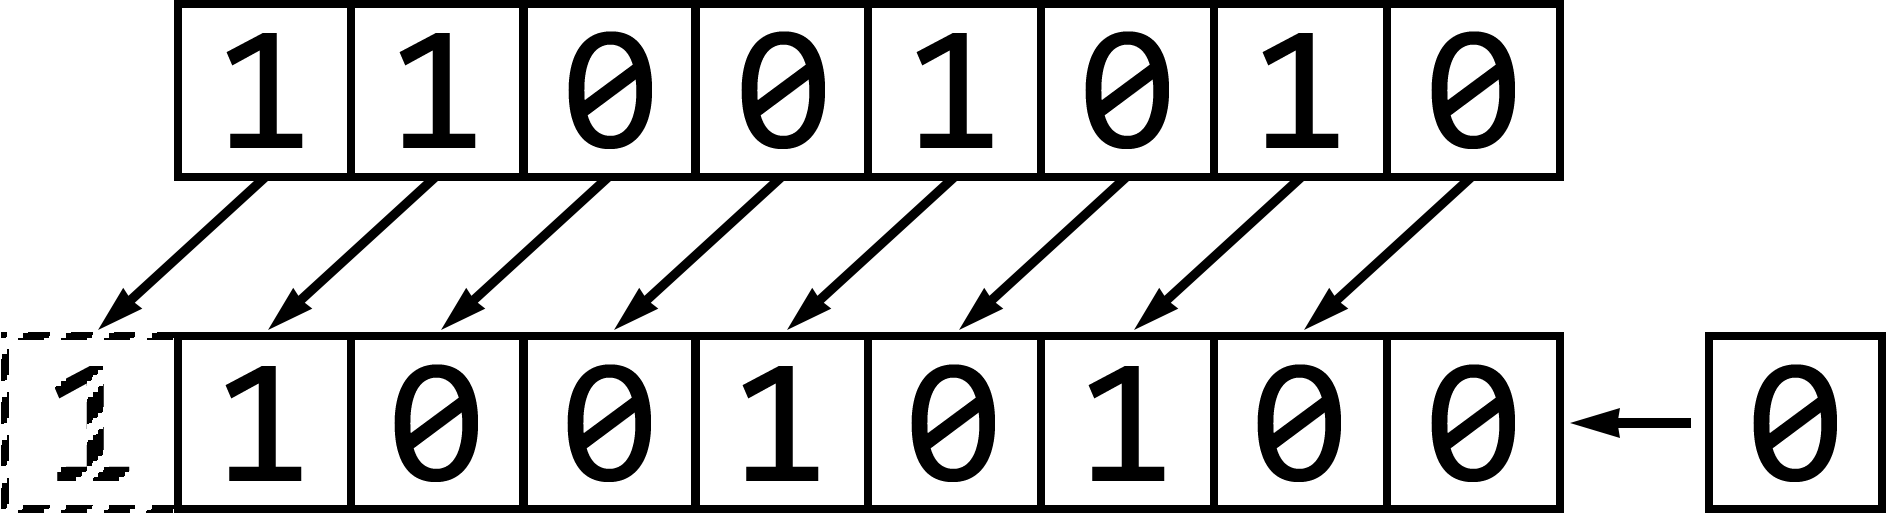
\includegraphics[width=9.69cm,height=2.75cm]{leftshift}
		\caption{Linksverschiebung} %\footnotemark}
		\label{fig:leftshift}
	\end{figure}
	\noindent
	Soll das MSB (höchstwertiges Bit) nicht verloren gehen, wird eine zirkuläre Linksverschiebung, dargestellt durch $\lll n$, angewandt. Dabei werden abgeschnittene Stellen hinten angehängt.
	
	\begin{figure}[!h]
		\vspace{.25cm}
		\centering
		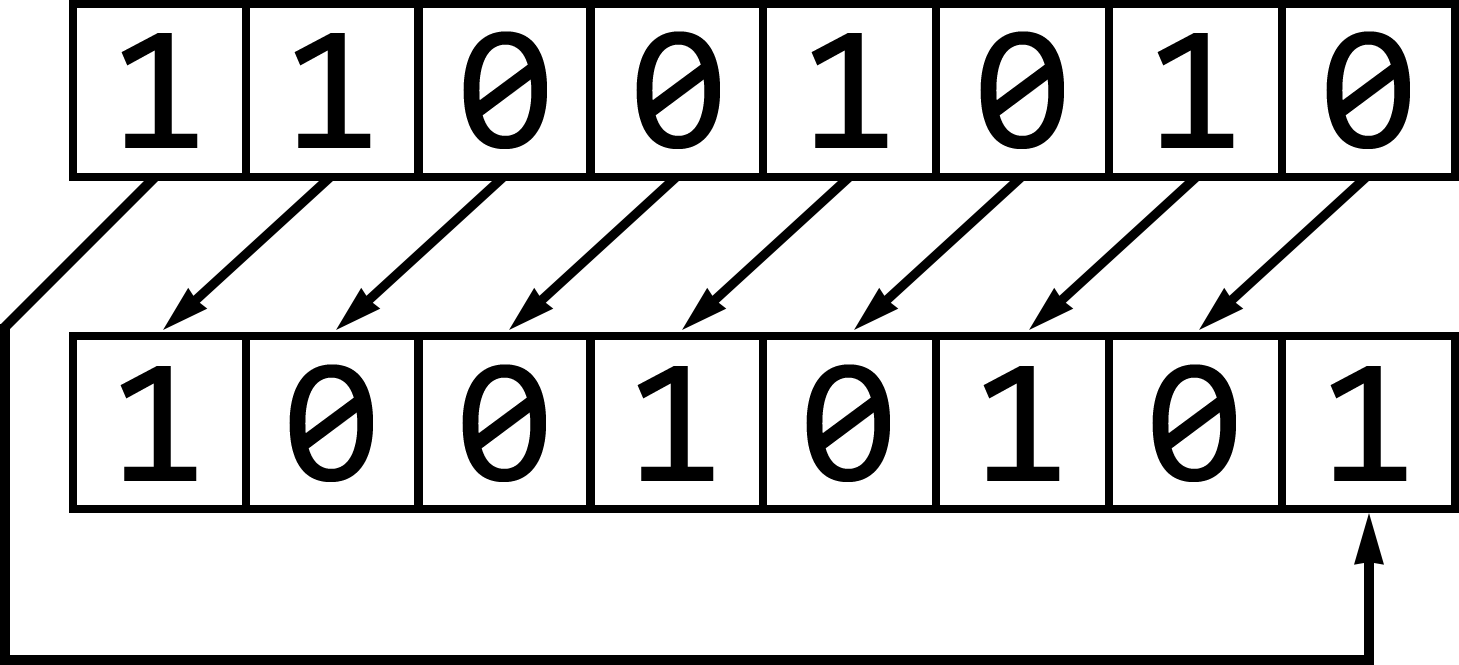
\includegraphics[width=7.5cm,height=3.56cm]{leftrot}
		\caption{Zirkuläre Linksverschiebung} %\footnotemark}
		\label{fig:leftrot}
	\end{figure}

	\subsection{Angriffe}
	Ein Hash Algorithmus gilt im kryptographischen Sinne als gebrochen, wenn es eine Methode oder einen Angriff gibt, der schneller eine Kollision herbeiführt als ein Brute Force Angriff.\autocite[vgl.][2]{schneierSelfStudy}
	
	\subsubsection{Preimage-Angriff}\label{preimage}
	Bei einem Preimage(Urbild)-Angriff wird versucht, eine Nachricht $x$ zu finden, die einen dem Angreifer bekannten Hashwert $z$ liefert, zum Beispiel um einen unterzeichneten Vertrag im Nachhinein zu ändern. \autocite[vgl.][5]{angriffAufMD5uSHA1}
	\begin{align*}
		h(x)=z
	\end{align*}
	\subsubsection{Second-Preimage-Angriff}
	Bei einem Second-Preimage-Angriff ist im Gegensatz zu \cref{preimage} nicht nur der Hashwert $z$ sondern auch die ursprüngliche Nachricht $x_1$, für die gilt $h(x_1) = z$, bekannt. Gesucht ist eine Nachricht $x_2\neq x_1$, für die
	\begin{align*}
		h(x_2)=h(x_1)
	\end{align*}
	gilt. \autocite[vgl.][S. 6 f.]{angriffAufMD5uSHA1}
	
	
	\subsubsection{Kollisionsangriff}
	Bei einem Kollisionsangriff werden zwei unterschiedliche Nachrichten $x_1\neq x_2$ gesucht, die  die Gleichung 
	\begin{align*}
		h(x_1) = h(x_2)
	\end{align*}
	erfüllen.\\
	Ein sehr naiver Ansatz wäre es, ein zufälliges $x_1$ zu wählen und danach einen second- Preimage-Angriff durchzuführen. Dabei wären bei einem 160 Bit langen Hashwert rund $2^{160}$ Berechnungen nötig, um mit großer Wahrscheinlichkeit eine Kollision zu finden. \\
	Mit Hilfe eines Geburtstagsangriffes kann mit weit weniger Berechnungen eine gleichgroße Erfolgswahrscheinlichkeit erreicht werden. Dabei werden $n$ zufällige Nachrichten $x_1,\dots ,x_n$ gewählt und für jede der Hashwert $z=h(x_i)$ berechnet. Danach wird überprüft, ob zwei Nachrichten denselben Hashwert ergeben haben. Analog zum Geburtstagsparadoxon lässt sich die Erfolgswahrscheinlichkeit bei $m$ möglichen Hashwerten, wie folgt, berechnen.
	\begin{align*}
	p=1-\left(\dfrac{m}{m} * \dfrac{m-1}{m}\cdots \dfrac{m-n+1}{m}\right)
	\end{align*}
	Um mit Wahrscheinlichkeit $\geq 1/2$ ein Kollision zu finden, sind $n\approx 1.17*\sqrt{m}$ Berechnungen notwendig. Um mit großer Wahrscheinlichkeit eine Kollision zu finden, sind $\approx 2^{80}$ Berechnungen nötig. \autocite[vgl.][S. 5 f.]{angriffAufMD5uSHA1}
	
	
	
	%angriff auf zertifikate!!
	
	
	%\subsection{Salt}
	\newpage
	\section{Hashfunktionen im Vergleich}\label{vergleich}
	\subsection{Message-Digest Algorithm 4 (MD4)}\label{md4}
	1990 veröffentlichte Ron Rivest MD4. Dieser orientiert sich am Merkel-Damg\aa rd-Prinzip, baut jedoch nicht auf anderen Bausteinen der Kryptographie (wie z.B. Blockchiffren) auf. Da MD4 nur einfache Bitmanipulationen mit 32-Bit-Operanden verwendet, eignet sich der Algorithmus für schnelle Softwareimplementierungen. Üblicherweise werden Bit-Strings, welche aus genau 32 Bit bestehen, als Wort bezeichnet. Weiters wird für Wörter $x,y$, $x +y$ als Addition modulo $2^{32}$ definiert. Die verwendeten Bit-Operatoren sind in \cref{bitoperatoren} beschrieben.\autocite[vgl.][S. 19~f.]{md4Familie}
	\par\noindent
	Die Funktionen $f,g$ und $h$ bilden auf Wörter ab und seien folgendermaßen definiert.
	\begin{align}
	f(x,y,z) &\coloneqq (x\wedge y) \vee ((\neg x)\wedge z)\\ \label{md4-f}
	g(x,y,z) &\coloneqq (x\wedge y) \vee (x\wedge z)\vee (y\wedge z)\\
	h(x,y,z) &\coloneqq x\oplus y \oplus z
	\end{align}


%\begin{table}[h!]
%	\centering
%	\begin{tabular}{|c|c|c|c|c|c|}
%		\hline
%		\rowcolor[HTML]{C0C0C0} 
%		{\color[HTML]{000000} x} & {\color[HTML]{000000} y} & {\color[HTML]{000000} z} & {\color[HTML]{000000} \begin{tabular}[c]{@{}c@{}}f\\ $(x\wedge y) \vee ((\neg x)\wedge z)$\end{tabular}} & {\color[HTML]{000000} \begin{tabular}[c]{@{}c@{}}g\\ $(x\wedge y) \vee (x\wedge z)\vee (y\wedge z)$\end{tabular}} & {\color[HTML]{000000} \begin{tabular}[c]{@{}c@{}}h\\ $x\oplus y \oplus z$\end{tabular}} \\ \hline
%		\rowcolor[HTML]{EFEFEF} 
%		0 & 0 & 0 & 0 & 0 & 0 \\ \hline
%		\rowcolor[HTML]{EFEFEF} 
%		0 & 0 & 1 & 1 & 0 & 1 \\ \hline
%		\rowcolor[HTML]{EFEFEF} 
%		0 & 1 & 0 & 0 & 0 & 1 \\ \hline
%		\rowcolor[HTML]{EFEFEF} 
%		0 & 1 & 1 & 1 & 1 & 0 \\ \hline
%		\rowcolor[HTML]{EFEFEF} 
%		1 & 0 & 0 & 0 & 0 & 1 \\ \hline
%		\rowcolor[HTML]{EFEFEF} 
%		1 & 0 & 1 & 0 & 1 & 0 \\ \hline
%		\rowcolor[HTML]{EFEFEF} 
%		1 & 1 & 0 & 1 & 1 & 0 \\ \hline
%		\rowcolor[HTML]{EFEFEF} 
%		1 & 1 & 1 & 1 & 1 & 1 \\ \hline
%	\end{tabular}
%	\caption{Wahrheitstafel für $f,g$ und $h$}
%\end{table}
	
	
	
	\mpar{1. Schritt (1-0-Padding)}\noindent
	Da sich MD4 am Merkel-Damg\aa rd-Prinzip orientiert, wird die Nachricht zunächst um einige Bits erweitert. An das Argument der Hashfunktion werden ein Einser und danach, falls nötig, so viele Nullen angehängt, bis die Länge des Bit-Strings kongruent 448 modulo 512 ist. Sollte die Länge der Nachricht bereits vor diesem Schritt kongruent 448 modulo 512 sein, wird sie um 512 Bit erweitert.\autocite[vgl.][20]{md4Familie}
	
	\mpar{2. Schritt (Längenpadding)}\noindent
	Anschließend wird die Länge der ursprünglichen Nachricht in Bit konkateniert\footnote{Als Konkatenation wird die Verkettung von Zeichen oder Zeichenketten bezeichnet.}. Dafür wird ein 64-Bit-String gebildet, um insgesamt eine Kongruenz 0 modulo 512 zu erreichen. Dabei wird der 64-Bit-String in 2 Wörter geteilt und das niederwertigere Wort zuerst angehängt. Sollte die Länge nicht als 64-Bit-String darstellbar sein, wird stattdessen die Kongruenz modulo $2^{64}$ konkateniert.\autocite[vgl.][21]{md4Familie}
	
	\mpar{3. Schritt (Initialisierung)}\noindent
	Der MD4 Hashalgorithmus verwendet einen 4-Wort-Puffer (A, B, C, D). Um die Werte A, B, C und D zwischen Durchläufen zu speichern, wird ein zweiter Puffer (AA, BB, CC, DD) benötigt. Die 32-Bit-Strings werden mit folgenden Hexadezimal-Werten initialisiert: \autocite[vgl.][S. 247~f.]{cryptography}
	\begin{align*}
		A &= 67452301\\
		B &= efcdab89\\
		C &= 98badcfe\\
		D &= 10325476
	\end{align*}

	\mpar{4. Schritt (Argumentverarbeitung)}\noindent
	Da dank der ersten beiden Schritte sichergestellt ist, dass die Länge der Nachricht $x$ (in Bit) ein ganzzahliges Vielfaches von 512 ist, kann nun der Vektor 
	\begin{align*}
		M = M[0]M[1]\dots M[N - 1]
	\end{align*}
	so gebildet werden, dass $M[i]$ ein 32-Bit-String ist und dass $N\equiv 0\mod 16$ ist.
	Anschließend wird die Nachricht in 512-Bit-Blöcken verarbeitet (je 16 $M$s). Die 16 aktuell verwendeten $M$s werden mit $X[0]\dots X[15]$ bezeichnet und die Werte von A, B, C und D in AA, BB, CC, DD gespeichert. Danach werden in drei sich voneinander unterscheidenden \textquotedblleft Runden\textquotedblright{} je 16 Operationen durchgeführt (zu jedem $X$ eine).\autocite[vgl.][S. 247~f.]{cryptography}\\

	\noindent \textbf{Runde 1}\par \label{round1-md4}\noindent
	Aus Platzgründen wird die Operation 
	\begin{align}
		a = (a + f(b,c,d) + X[k])\lll s \label{operation1-md4}
	\end{align}
	im Folgenden durch [abcd k s] repräsentiert. Es wird
	\vspace{.5cm}
	\newline
	[ABCD \:\:0 3],\hfill [DABC \:\:1 7],\hfill [CDAB \:\:2 11],\hfill [BCDA \:\:3 19],
	\newline
	[ABCD \:\:4 3],\hfill [DABC \:\:5 7],\hfill [CDAB \:\:6 11],\hfill [BCDA \:\:7 19],
	\newline
	[ABCD \:\:8 3],\hfill [DABC \:\:9 7],\hfill [CDAB 10 11],\hfill [BCDA 11 19],
	\newline
	[ABCD 12 3],\hfill [DABC 13 7],\hfill [CDAB 14 11],\hfill [BCDA 15 19]\:
	\spar
	ausgeführt.\\
	\vspace{.5cm}
	
	\noindent \textbf{Runde 2}\par\noindent
	Im Folgenden wird die Operation 
	\begin{align}
	a = (a + g(b,c,d) + X[k] + 5a827999)\lll s
	\end{align}
	durch [abcd k s] repräsentiert. Im Gegensatz zu Runde eins wird nun eine additive Konstante, $5a827999$(hex), verwendet. Es wird
	\vspace{.5cm}
	\newline
	[ABCD 0 3],\hfill [DABC 4 5],\hfill [CDAB \:\:8 9],\hfill [BCDA 12 13],
	\newline
	[ABCD 1 3],\hfill [DABC 5 5],\hfill [CDAB \:\:9 9],\hfill [BCDA 13 13],
	\newline
	[ABCD 2 3],\hfill [DABC 6 5],\hfill [CDAB 10 9],\hfill [BCDA 14 13],
	\newline
	[ABCD 3 3],\hfill [DABC 7 5],\hfill [CDAB 11 9],\hfill [BCDA 15 13]\:
	\spar
	ausgeführt.\\
	\vspace{.5cm}
	
	
	\noindent \textbf{Runde 3}\par\noindent
	Im Folgenden wird die Operation 
	\begin{align}
	a = (a + h(b,c,d) + X[k] + 6ed9eba1)\lll s
	\end{align}
	durch [abcd k s] repräsentiert. Es wird eine additive Konstante, $6ed9eba1$(hex), verwendet. Es wird
	\vspace{.5cm}
	\newline
	[ABCD 0 3],\hfill [DABC \:\:8 9],\hfill [CDAB 4 11],\hfill [BCDA 12 15],
	\newline
	[ABCD 2 3],\hfill [DABC 10 9],\hfill [CDAB 6 11],\hfill [BCDA 14 15],
	\newline
	[ABCD 1 3],\hfill [DABC \:\:9 9],\hfill [CDAB 5 11],\hfill [BCDA 13 15],
	\newline
	[ABCD 3 3],\hfill [DABC 11 9],\hfill [CDAB 7 11],\hfill [BCDA 15 15]\:
	\spar
	ausgeführt.\\
	\vspace{.5cm}
\noindent
	Nach der dritten Runde werden die Pufferwerte A, B, C und D durch A + AA, B + BB, C + CC und D + DD ersetzt. Diese drei Runden werden für jeden 512-Bit-Block der Nachricht wiederholt. \autocite[vgl.][S. 4 f.]{rivest}
	
	\mpar{5. Schritt (Ausgabe)}\noindent
	Nachdem alle Blöcke verarbeitet wurden, ergibt die Konkatenation $A\parallel B\parallel C\parallel D$ den 128-Bit-Hashwert.
	
	\subsubsection{Beispiel}
	Die Nachricht $x$ sei durch den 56-Bit-String 
	\begin{align*}
		 01100010~01100011~01110010~01111001~01110000~01110100~00111111
		%01101101~01100100~00110100~00101101~01100110~01110100~01110111
	\end{align*}
	repräsentiert.\\
	\noindent \textbf{1. Schritt}\par\noindent
	Die Nachricht $x$ wird zu
	\begin{align*}
	~~01100010~01100011~01110010~01111001~01110000~01110100~00111111~1
	\end{align*}
	erweitert.\\
	\noindent \textbf{2. Schritt}\par\noindent
	Die Länge $L$, der Nachricht $x$ ist nach dem ersten Schritt 57. Es werden $K=391$ Nullen angehängt, was folgenden Hexadezimal-Wert ergibt.
	\begin{align*}
	&62637279~70743f80~00000000~00000000\\
	&00000000~00000000~00000000~00000000\\
	&00000000~00000000~00000000~00000000\\
	&00000000~00000000
	\end{align*}
	\\
	\noindent \textbf{3. Schritt}\par\noindent
	Die 64-Bit-Darstellung von L = 56 ist $00000000~00000038$(hex). Der 64-Bit-String wird an die Nachricht angehängt.
	\begin{align*}
	&62637279~70743f80~00000000~00000000\\
	&00000000~00000000~00000000~00000000\\
	&00000000~00000000~00000000~00000000\\
	&00000000~00000000~00000000~00000038
	\end{align*}
	\\
	\noindent \textbf{4. Schritt}\par\noindent
	Da die Nachricht nun genau 512 Bit lang ist, wird nur ein Durchlauf der Hauptschleife benötigt. Die Nachricht wird in 16 32-Bit-Blöcke geteilt.
	\begin{align*}
	X[0] &= 62637279\\
	X[1] &= 70743f80\\
	\vdots \\
	X[14] &= 00000000\\
	X[15] &= 00000038
	\end{align*}
	Nun sind die in \cref{round1-md4} beschriebenen Operationen der ersten Runde auszuführen. Dafür wird in \eqref{operation1-md4} eingesetzt.
	\begin{align*}
	A = (67452301 + f(efcdab89, 98badcfe, 10325476) + X[0])\lll 3
	\end{align*}
	Um den Rückgabewert von $f(efcdab89, 98badcfe, 10325476)$ zu berechnen, muss in \eqref{md4-f} eingesetzt werden.
	\begin{align*}
		f(efcdab89, 98badcfe, 10325476) = (efcdab89\wedge 98badcfe) \vee ((\neg efcdab89)\wedge 10325476)		
	\end{align*}
	Nun  werden die einzelnen Bitmanipulationen durchgeführt. Dafür werden die Hexadezimal-Werte als 32-Bit-Strings dargestellt.\\
	Die erste Klammer:
	\begin{align*}
		&1110~1111~1100~1101~1010~1011~1000~1001\\
	\BitAnd~&1001~1000~1011~1010~1101~1100~1111~1110\\
		=~&1000~1000~1000~1000~1000~1000~1000~1000
	\end{align*}
	Die zweite Klammer:
	\begin{align*}
		&0001~0000~0011~0010~0101~0100~0111~0110\\
	\BitAnd~&0001~0000~0011~0010~0101~0100~0111~0110\\
		=~&0001~0000~0011~0010~0101~0100~0111~0110
	\end{align*}
	Das Endergebnis:
	\begin{align*}
		&1000~1000~1000~1000~1000~1000~1000~1000\\
	 \BitOr~&0001~0000~0011~0010~0101~0100~0111~0110\\
		=~&1001~1000~1011~1010~1101~1100~1111~1110
	\end{align*}
	\noindent
	Anschließend wird der errechnete Wert mit $67452301$(hex) und $X[0]$ modulo $2^{32}$ addiert.
	\begin{align*}
	67452301 + 98badcfe + 62637279 = 162637279\\
	162637279 \equiv 62637279\mod 100000000
	\end{align*}
	\noindent
	Zuletzt wird nun eine zirkuläre Linksverschiebung um 3 Bit durchgeführt.
	
	\begin{align*}
	&0110~0010~0110~0011~0111~0010~0111~1001\lll 3\\
	=~&0001~0011~0001~1011~1001~0011~1100~1011
	\end{align*}
	\noindent
	Der Pufferwert A wird durch 
	\begin{align*}
		A = 131b93cb
	\end{align*}
	ersetzt.
	
	\par\noindent
	Wie zu sehen ist, sind die Startwerte des Puffers (A, B, C, D) so gewählt, dass der Wert A in der ersten Operation der ersten Runde durch den um 3 Bit zirkulär linksverschobenen Wert des Wortes $X[0]$  ersetzt wird.\\ Nach dem Durchlaufen aller drei Runden ergibt sich der Hashwert 
	\begin{align*}
		h(x)=993ec669ce8c97edf20d01c37f090538
	\end{align*} 
	
	
	
		
		
	\subsubsection{Erfolgreiche Angriffe}
	Bereits kurze Zeit nach seiner Veröffentlichung wurden Schwächen im MD4 Algorithmus entdeckt, weshalb 1991 MD5 veröffentlicht wurde.
	\mpar{1995}\noindent
	 1995 gelang es Hans Dobbertin einen Angriff auf zwei der drei Runden von RIPEMD\footnote{Bei RIPEMD handelt es sich um eine von Hans Dobbertin entworfene Hashfunktion.} zu finden.  Durch eine Abstraktion dieses Angriffes konnte er erstmalig einen erfolgreichen Angriff auf den gesamten MD4 Algorithmus demonstrieren. Der Angriff benötigt nur wenige Sekunden auf einem einfachen PC (1995). In seinem Paper stellt er sogar in Frage, ob MD4 eine Einwegfunktion ist, da es sehr schnell möglich ist, einen Urbild-Angriff auf die ersten beiden Runden von MD4 durchzuführen.\autocite[vgl.][1]{dobbertin}
	\mpar{2004}\noindent
	2004 gelang es dem chinesischen Forscherteam rund um Xiaoyun Wang einen Weg zu finden, auch ohne Computer Kollisionen zu finden. Es ist lediglich die Berechnung von
	\begin{align*}
		M' = M + \Delta C, \Delta C = (0,2^{31},-2^{28}+2^{31},0,0,0,0,0,0,0,0,0,-2^{16},0,0,0)
	\end{align*}
	nötig, damit $MD4(M) = MD4(M')$ ist.\autocite[vgl.][3]{md4Collision}\\
	\noindent
	\begin{table}[h!]
	\begin{tabular}{|c|c|}
		\hline 
		$M_1$ & 4d7a9c83\hfill{} 56cb927a\hfill{}  b9d5a578\hfill{} 57a7a5ee\hfill{} de748a3c\hfill{} dcc366b3\hfill{} b683a020\hfill{} 3b2a5d9f\\
		& c69d71b3\hfill{} f9e99198\hfill{} d79f805e\hfill{} a63bb2e8\hfill{} 45dd8e31\hfill{} 97e31fe5\hfill{} 2794bf08\hfill{} b9e8c3e9\\ 
		\hline 
		$M_1$ & 4d7a9c83\hfill{} d6cb927a\hfill{} 29d5a578\hfill{} 57a7a5ee\hfill{} de748a3c\hfill{} dcc366b3\hfill{} b683a020\hfill{} 3b2a5d9f\\
		& c69d71b3\hfill{} f9e99198\hfill{} d79f805e\hfill{} a63bb2e8\hfill{} 45dc8e31\hfill{} 97e31fe5\hfill{} 2794bf08\hfill{} b9e8c3e9\\ 
		\hline 
		$H$ & \multicolumn{1}{l|}{5f5c1a0d 71b36046 1b5435da 9b0d807a} \\ 
		\hline
		$M_2$ & 4d7a9c83\hfill{} 56cb927a\hfill{} b9d5a578\hfill{} 57a7a5ee\hfill{} de748a3c\hfill{} dcc366b3\hfill{} b683a020\hfill{} 3b2a5d9f\\
		& c69d71b3\hfill{} f9e99198\hfill{} d79f805e\hfill{} a63bb2e8\hfill{} 45dd8e31\hfill{} 97e31fe5\hfill{} f713c240\hfill{} a7b8cf69\\
		\hline 
		$M_2$ & 4d7a9c83\hfill{} d6cb927a\hfill{} 29d5a578\hfill{} 57a7a5ee\hfill{} de748a3c\hfill{} dcc366b3\hfill{} b683a020\hfill{} 3b2a5d9f\\
		& c69d71b3\hfill{} f9e99198\hfill{} d79f805e\hfill{} a63bb2e8\hfill{} 45dc8e31\hfill{} 97e31fe5\hfill{} f713c240\hfill{} a7b8cf69\\
		\hline 
		$H$ & \multicolumn{1}{l|}{e0f76122 c429c56c ebb5e256 b809793} \\ 
		\hline 
	\end{tabular} 
\caption{Je zwei Nachrichten, die unter MD4 kollidieren \autocite[3]{md4Collision}}
\end{table}

	\newpage
	\subsection{Message-Digest Algorithm 5 (MD5)}
	Bei MD5 handelt es sich um eine verbesserte Version von MD4. Als es Boer, Bosselaers und Merkel gelang, erfolgreich die ersten zwei Runden(Merkel) bzw. die letzten beiden Runden (Boer und Bosselaers) von MD4 anzugreifen, veröffentlichte Rivest 1991 MD5. Dies geschah noch bevor Angriffe auf MD4 bekannt waren.\autocite[vgl.][498]{angewandteKryptographie}\par\noindent
	Da bei MD5 (im Gegensatz zu MD4) vier Runden durchgeführt werden, werden vier nichtlineare Funktionen benötigt. Es sei
	\begin{align}
		f(x, y, z) &\coloneqq (x\wedge y)\vee ((\neg x)\wedge z)\\
		g(x, y, z) &\coloneqq (x\wedge y)\vee (y\wedge (\neg z))\label{g-md5}\\ 
		h(x, y, z) &\coloneqq x\oplus y\oplus z\\
		i(x, y, z) &\coloneqq y\oplus (x\vee (\neg z))
	\end{align}
	definiert.\par\noindent
	Die ersten drei Schritte unterscheiden sich nicht von den in \cref{md4} beschriebenen.
	\mpar{1.Schritt (1-0-Padding)}
	\mpar{2.Schritt (Längenpadding)}
	\mpar{3.Schritt (Initialisierung)}	
	\mpar{4.Schritt (Argumentverarbeitung)}\noindent
	Wie in MD4 wird der Eingabetext in Blöcken zu je 512 Bit, aufgeteilt in 16 Teilblöcke der Länge 32 Bit, verarbeitet. Die 16 aktuellen Teilblöcke werden erneut mit $X[0]\dots X[15]$ bezeichnet.
	Weiters benötigt MD5 64 konstante Wörter, die im Folgenden mit $T[1]\dots T[64]$ bezeichnet werden. $T[i]$ bezeichnet den ganzzahlige Teil von $2^{32}|sin(i)|$, wobei $i$ im Bogenmaß gemessen wird.  
	\par\noindent
	Die Werte von A, B, C und D werden in AA, BB, CC, DD gespeichert. Danach werden in vier sich leicht voneinander unterscheidenden \textquotedblleft Runden\textquotedblright{} je 16 Operationen durchgeführt. \autocite[vgl.][4]{rivest}\\
	
	\noindent \textbf{Runde 1}\par\noindent
	Die Operation 
	\begin{align*}
	a = b+ ((a + f(b,c,d) + X[k] + T[i])\lll s)
	\end{align*}
	wird durch [abcd k s i] repräsentiert. Es wird
	\vspace{.5cm}
	\newline
	[ABCD \:\:0 7 \:\:1],\hfill [DABC \:\:1 12 \:\:2],\hfill [CDAB \:\:2 17 \:\:3],\hfill [BCDA \:\:3 22 \:\:4],
	\newline
	[ABCD \:\:4 7 \:\:5],\hfill [DABC \:\:5 12 \:\:6],\hfill [CDAB \:\:6 17 \:\:7],\hfill [BCDA \:\:7 22 \:\:8],
	\newline
	[ABCD \:\:8 7 \:\:9],\hfill [DABC \:\:9 12 10],\hfill [CDAB 10 17 11],\hfill [BCDA 11 22 12],
	\newline
	[ABCD 12 7 13],\hfill [DABC 13 12 14],\hfill [CDAB 14 17 15],\hfill [BCDA 15 22 16]\:
	\spar
	ausgeführt.\\
	\vspace{.5cm}
	
	\noindent \textbf{Runde 2}\par\noindent
	Die Operation 
	\begin{align*}
	a = b+ ((a + g(b,c,d) + X[k] + T[i])\lll s)
	\end{align*}
	wird durch [abcd k s i] repräsentiert. Es wird
	\vspace{.5cm}
	\newline
	[ABCD \:\:1 5 17],\hfill [DABC \:\:6 9 18],\hfill [CDAB 11 14 19],\hfill [BCDA \:\:0 20 20],
	\newline
	[ABCD \:\:5 5 21],\hfill [DABC 10 9 22],\hfill [CDAB 15 14 23],\hfill [BCDA \:\:4 20 24],
	\newline
	[ABCD \:\:9  5 25],\hfill [DABC 14 9 26],\hfill [CDAB \:\:3 14 27],\hfill [BCDA \:\:8 20 28],
	\newline
	[ABCD 13 5 29],\hfill [DABC \:\:2 9 30],\hfill [CDAB \:\:7 14 31],\hfill [BCDA 12 20 32]\:
	\spar
	ausgeführt.\\
	\vspace{.5cm}
	
	\noindent \textbf{Runde 3}\par\noindent
	Die Operation 
	\begin{align*}
	a = b+ ((a + h(b,c,d) + X[k] + T[i])\lll s)
	\end{align*}
	wird durch [abcd k s i] repräsentiert. Es wird
	\vspace{.5cm}
	\newline
	[ABCD \:\:5 4 33],\hfill [DABC \:\:8 11 34],\hfill [CDAB 11 16 35],\hfill [BCDA 14 23 36],
	\newline
	[ABCD \:\:1 4 37],\hfill [DABC \:\:4 11 38],\hfill [CDAB \:\:7 16 39],\hfill [BCDA 10 23 40],
	\newline
	[ABCD 13  4 41],\hfill [DABC \:\:0 11 42],\hfill [CDAB \:\:3 16 43],\hfill [BCDA \:\:6 23 44],
	\newline
	[ABCD \:\:9 4 45],\hfill [DABC 12 11 46],\hfill [CDAB 15 16 47],\hfill [BCDA \:\:2 23 48]\:
	\spar
	ausgeführt.\\
	\vspace{.5cm}
	
	\noindent \textbf{Runde 4}\par\noindent
	Die Operation 
	\begin{align*}
	a = b+ ((a + i(b,c,d) + X[k] + T[i])\lll s)
	\end{align*}
	wird durch [abcd k s i] repräsentiert. Es wird
	\vspace{.5cm}
	\newline
	[ABCD \:\:0 6 49],\hfill [DABC \:\:7 10 50],\hfill [CDAB 14 15 51],\hfill [BCDA \:\:5 21 52],
	\newline
	[ABCD 12 6 53],\hfill [DABC \:\:3 10 53],\hfill [CDAB 10 15 55],\hfill [BCDA \:\:1 21 56],
	\newline
	[ABCD \:\:8  6 57],\hfill [DABC 15 10 58],\hfill [CDAB \:\:6 15 59],\hfill [BCDA 13 21 60],
	\newline
	[ABCD \:\:4 6 61],\hfill [DABC 11 10 62],\hfill [CDAB \:\:2 15 63],\hfill [BCDA \:\:9 21 64]\:
	\spar
	ausgeführt.\autocite[vgl.][5]{rivest}\\
	\vspace{.5cm}
	\noindent
	Nach der dritten Runde werden die Pufferwerte A, B, C und D durch A + AA, B + BB, C + CC und D + DD ersetzt.\par\noindent
	Diese drei Runden werden für jeden 512-Bit-Block der Nachricht wiederholt.
	
	\mpar{5. Schritt (Ausgabe)}\noindent
	Nachdem alle Blöcke verarbeitet wurden, ergibt die Konkatenation $A\parallel B\parallel C\parallel D$ den 128-Bit-Hashwert.
	
	\subsubsection{Unterschiede zu MD4}
	Ron Rivest beschreibt die Änderungen von MD5 wie folgt\autocite[S. 502~f.]{angewandteKryptographie}:
	\begin{itemize}
		\item[1.] Eine vierte Runde wurde hinzugefügt.
		\item[2.] Jeder Schritt enthält jetzt eine eindeutige additive Konstante.
		\item[3.] Die Funktion G in Runde 2 wurde von $(x\wedge y) \vee (x\wedge z)\vee (y\wedge z)$ zu $(x\wedge y)\vee (y\wedge (\neg z))$ geändert, um G weniger symmetrisch zu machen.\footnote{mit G ist g in \eqref{g-md5} gemeint}
		\item[4.] In jedem Schritt wird jetzt das Ergebnis des vorherigen Schrittes addiert. Dies liefert einen schnelleren Lawineneffekt\footnote{Bei einer minimalen Änderung der Eingabe, ändert sich die Ausgabe völlig.}.
		\item[5.] Die Reihenfolge, in der in den Runden 2 und 3 auf die Teilblöcke zugegriffen wird, wurde geändert, um ähnliche Muster zu vermeiden.
		\item[6.] Die Beträge der zirkulären Linksverschiebungen in jeder Runde wurden optimiert, um einen schnelleren Lawineneffekt zu erreichen. Die vier Verschiebungen in den einzelnen Runden unterscheiden sich von denen in den anderen Runden.
	\end{itemize}
\newpage
\subsubsection{Erfolgreiche Angriffe}
	\mpar{1993}\noindent
		1993 gelang es Bert den Boer und Antoon Bosselaers einen Algorithmus zu entwickeln, um Kollisionen für die in MD5 verwendete Kompressionsfunktion der ersten beiden Runden zu finden. Der Angriff stützt sich auf eine der zwei Änderungen, die Rivest vornahm, um MD5 sicherer zu machen als MD4. \autocite[vgl.][1]{boer}
		
	\mpar{1996}\noindent
	Hans Dobbertin gelang es zwei 512-Bit-Strings zu finden, welche unter einer veränderten Version von MD5 kollidieren. Die Änderung beschränkt sich auf die Initialisierung der Puffer-Werte. Obwohl dies keine Auswirkungen auf den echten MD5 Algorithmus hat, zeigt es die Schwächen von MD5 auf.\autocite[vgl.][1]{md4Collision}
		
	\mpar{2004}\noindent
		Wang und seinem Team gelang es einen Weg zu finden, um Kollisionen zu errechnen. Dafür wird für eine 1024-Bit Nachricht $(M,N_i)$
		\begin{align*}
			M'&=M+\Delta C_1,\Delta C_1 = (0,0,0,0,2^{31},\dots ,2^{15},0,0,2^{31},0)\\
			N'_i &= N_i + \Delta C_2,\Delta C_2 = (0,0,0,0,2^{31},\dots ,-2^{15},0,0,2^{31},0)
		\end{align*}
		berechnet, sodass $MD5(M,N_i) = MD5(M',N'_i)$ ist.
		
		% Please add the following required packages to your document preamble:
		% \usepackage{multirow}
		\begin{table}[h!]
			\centering
			\begin{tabular}{|c|c|c|}
				\hline
				\multirow{2}{*}{$X_1$} & $M$   & \begin{tabular}[c]{@{}c@{}}2dd31d1\hfill{} c4eee6c5\hfill{} 69a3d69\hfill{} 5cf9af98\hfill{} 87b5ca2f\hfill{} ab7e4612\hfill{} 3e580440\hfill{} 897ffbb8\\ 634ad55\hfill{} 2b3f409\hfill{} 8388e483\hfill{} 5a417125\hfill{} e8255108\hfill{} 9fc9cdf7\hfill{} f2bd1dd9\hfill{} 5b3c3780\end{tabular}    \\ \cline{2-3} 
				& $N_1$ & \begin{tabular}[c]{@{}c@{}}d11d0b96\hfill{} 9c7b41dc\hfill{} f497d8e4\hfill{} d555655a\hfill{} c79a7335\hfill{} cfdebf0\hfill{} 66f12930\hfill{} 8fb109d1\\ 797f2775\hfill{} eb5cd530\hfill{} baade822\hfill{} 5c15cc79\hfill{} ddcb74ed\hfill{} 6dd3c55f\hfill{} d80a9bb1\hfill{} e3a7cc35\end{tabular} \\ \hline
				\multirow{2}{*}{$X_1$} & $M'$  & \begin{tabular}[c]{@{}c@{}}2dd31d1\hfill{} c4eee6c5\hfill{} 69a3d69\hfill{} 5cf9af98\hfill{} 7b5ca2f\hfill{} ab7e4612\hfill{} 3e580440\hfill{} 897ffbb8\\ 634ad55\hfill{} 2b3f409\hfill{} 8388e483\hfill{} 5a41f125\hfill{} e8255108\hfill{} 9fc9cdf7\hfill{} 72bd1dd9\hfill{} 5b3c3780\end{tabular}     \\ \cline{2-3} 
				& $N_1$ & \begin{tabular}[c]{@{}c@{}}d11d0b96\hfill{} 9c7b41dc\hfill{} f497d8e4\hfill{} d555655a\hfill{} 479a7335\hfill{} cfdebf0\hfill{} 66f12930\hfill{} 8fb109d1\\ 797f2775\hfill{} eb5cd530\hfill{} baade822\hfill{} 5c154c79\hfill{} ddcb74ed\hfill{} 6dd3c55f\hfill{} 580a9bb1\hfill{} e3a7cc35\end{tabular} \\ \hline
				\multicolumn{2}{|c|}{$H$}      & \multicolumn{1}{l|}{9603161f f41fc7ef 9f65ffbc a30f9dbf}                                                                                                                                                                                                                                    \\ \hline
			\end{tabular}
			\caption{Zwei Nachrichten, die unter MD5 kollidieren \autocite[3]{md4Collision}}
			\label{md5-collision}
		\end{table}
		
	
	
	
	\newpage
	\subsection{Secure Hash Algorithm (SHA-1)}
	Von der NSA in Zusammenarbeit mit dem NIST entwickelt, sollte SHA-1 die im SHS (Secure Hash Standard) verwendete Hashfunktion sein. SHA-1 ist wie MD5 eine Verbesserung/Weiterentwicklung des MD4 Algorithmus. SHA-1 erzeugt für jede Eingabe $<2^{64}$ Bit einen 160 Bit langen Hashwert. Es werden vier Runden verwendet. Es seien dabei $f_1,f_2,f_3,f_4$ wie folgt definiert:\autocite[vgl.][504]{angewandteKryptographie}
	\begin{align*}
	f_1(x, y, z) &\coloneqq (x\wedge y)\vee ((\neg x)\wedge z)\\
	f_2(x, y, z) &\coloneqq x\oplus y\oplus z\\
	f_3(x, y, z) &\coloneqq (x\wedge y)\vee (y\wedge (\neg z))\\ 
	f_4(x, y, z) &\coloneqq x\oplus y\oplus z
	\end{align*}
	
	\mpar{1.Schritt (1-0-Padding)}\noindent
	Dieser Schritt unterscheidet sich nicht von dem in \cref{md4} beschriebenen.
	\mpar{2.Schritt (Längenpadding)}\noindent
	Die Länge der ursprünglichen Nachricht in Bit wird als 64-Bit-String angehängt. Im Gegensatz zu MD4 wird jedoch das höherwertige Wort zuerst konkateniert. \autocite[vgl.][S. 26 f.]{md4Familie}
	\mpar{3.Schritt (Initialisierung)}\noindent
	Da SHA-1 einen 160 Bit langen Hashwert liefert, werden zwei fünf 5-Wort-Puffer benötigt. Die fünf Puffervariablen werden wie folgt initialisiert. \autocite[vgl.][S. 505 f.]{angewandteKryptographie}
	\begin{align*}
		A&=67452310\\
		B&=efcdab89\\
		C&=98badcfe\\
		D&=10325476\\
		E&=c3d2e1f0
	\end{align*}
	
	\mpar{4.Schritt (Argumentverarbeitung)}\noindent
	Der Eingabetext wird in 512-Bit-Blöcken verarbeitet. Jeder Block wird in 16 Teilblöcke gespalten, welche mit $M[0]\dots M[15]$ bezeichnet werden. Die 16 $M$s werden in 80 32-Bit-Strings umgewandelt. 
	\begin{align*}
		W_t &= M_t	\text{~~~~~für $t$ = 0,\dots , 15}\\
		W_t &= (W_{t-3}\oplus W_{t-8}\oplus W_{t-14}\oplus W_{t-16})\lll 1 \text{~~~~~für $t$ = 16,\dots ,79}
	\end{align*}
	Weiters werden vier additive Konstanten benötigt.
	\begin{align*}
		K_1&=\dfrac{\sqrt{2}}{4} = 5a827999\\
		K_2&=\dfrac{\sqrt{3}}{4} = 6ed9eba1\\
		K_3&=\dfrac{\sqrt{5}}{4} = 8f1bbcdc\\
		K_4&=\dfrac{\sqrt{10}}{4} = ca62c1d6
	\end{align*}
	\noindent
	Die Hauptschleife besteht aus vier Runden zu je 20 Operationen und wird für jeden 512-Bit-Block durchlaufen.\par\noindent
	Zunächst werden die Variablen $A,B,C,D$ und $E$ in $a,b,c,d$ und $e$ gespeichert. Danach werden die vier Runden durchgeführt:\\
	\newline

	\noindent \textbf{Runde 1}\par
		\begin{align*}
			\text{Für $t = 0,\dots ,19$}\\
				TEMP &= (a\lll 5) + f_1(b,c,d) + e + W_t + K_1\\
				e&=d\\
				d&=c\\
				c&=b\lll 30\\
				b&=a\\
				a&=TEMP
		\end{align*}

	\noindent \textbf{Runde 2}\par
	\begin{align*}
	\text{Für $t = 20,\dots ,39$}\\
	TEMP &= (a\lll 5) + f_2(b,c,d) + e + W_t + K_2\\
	e&=d\\
	d&=c\\
	c&=b\lll 30\\
	b&=a\\
	a&=TEMP
	\end{align*}\newpage

	
	\noindent \textbf{Runde 3}\par
	\begin{align*}
	\text{Für $t = 40,\dots ,59$}\\
	TEMP &= (a\lll 5) + f_3(b,c,d) + e + W_t + K_3\\
	e&=d\\
	d&=c\\
	c&=b\lll 30\\
	b&=a\\
	a&=TEMP
	\end{align*}

	\noindent \textbf{Runde 4}\par
	\begin{align*}
	\text{Für $t = 60,\dots ,79$}\\
	TEMP &= (a\lll 5) + f_4(b,c,d) + e + W_t + K_4\\
	e&=d\\
	d&=c\\
	c&=b\lll 30\\
	b&=a\\
	a&=TEMP
	\end{align*}
\newline
	Die Variablen $a,b,c,d$ und $e$ werden zu $A,B,C,D$ und $E$ addiert und die Hauptschleife wird für den nächsten Block wiederholt.\autocite[vgl.][S. 505 f.]{angewandteKryptographie}\\\par\noindent
	Durch die Verschiebung der Variablen erreicht der Algorithmus das Gleiche wie MD5 durch die Verwendung verschiedener Variablen an verschiedenen Stellen.\autocite[506]{angewandteKryptographie}
	
	\mpar{5. Schritt (Ausgabe)}\noindent
	Nachdem alle Blöcke verarbeitet wurden, ergibt die Konkatenation $A\parallel B\parallel C\parallel D\parallel E$ den 160-Bit langen Hashwert.
	\newpage
	\subsubsection{Vergleich zu MD5}
	Sowohl bei MD5 als auch bei SHA handelt es sich um Weiterentwicklungen des MD4 Algorithmus. Die Verbesserungen unterscheiden sich in folgenden Punkten: \autocite[vgl.][507]{angewandteKryptographie}
	\begin{itemize}
		\item[1.]
		Sowohl bei MD5 als auch bei SHA wurde eine vierte Runde hinzugefügt.
		\item[2.]
		Während in MD5 jeder Schritt eine eindeutige additive Konstante enthält, behält SHA das Schema von MD4 bei. Je eine Konstante pro Runde.
		\item[3.]
		SHA behält die alte Funktion $g$ bei. MD5 hat diese durch $((X\wedge Y)\vee (Y\wedge(\neg Z)))$ ersetzt.
		\item[4.]
		Sowohl bei SHA als auch bei MD5 wird in jedem Schritt das Ergebnis des vorherigen Schrittes addiert. SHA verwendet dafür eine fünfte Variable, was den Angriff von Boer und Bosselaers auf MD5 verhindert.
		\item[5.]
		\textquotedblleft Die Reihenfolge, in der in Runde zwei und drei auf die Teilblöcke zugegriffen wird, wurde geändert, um ähnliche Muster zu vermeiden\textquotedblright{} SHA ist völlig anders, da es einen zyklisch fehlerkorrigierten Code benutzt.\autocite[507]{angewandteKryptographie}
		\item[6.]
		Bei MD5 wurden die Beträge der Linksverschiebung für einen schnelleren Lawineneffekt optimiert. SHA verschiebt in jeder Runde um einen konstanten Betrag.
	\end{itemize}
\subsubsection{Erfolgreiche Angriffe}
	\mpar{2005}\noindent
	2005 gelang es den Wissenschaftlern Xiaoyun Wang, Yiqun Lisa Yin und Hongbo Yu erstmals SHA-1 zu brechen. Kollisionen können mit nur $2^{69}$ Berechnungen gefunden werden. Das ist mehr als 2000-mal schneller als Bruteforce. \autocite[vgl.][]{sha1Broken}
	\mpar{2015}\noindent
	2015 ist erstmals ein nicht nur theoretischer Angriff auf SHA-1 gelungen. Die Forscher Marc Stevens, Pierre Karpman und Thomas Peyrin haben eine Freestart-Kollision, für die in SHA-1 verwendete Kompressionsfunktion, gefunden.\\\autocite[vgl.][]{sha1Collision}\\
	\newline
	Bis heute wurde keine Kollision für SHA-1 veröffentlicht.
	
	%\subsection{Lan Manager (LM)}
	\newpage
	\section{Angriffe auf Passwörter}\label{angriffe}
	In der Praxis werden Hashfunktionen oft für die Sicherung von Passwörtern verwendet. Ziel ist es, die beim Hack einer Datenbank gestohlenen Passwörter für Angreifer unbrauchbar zu machen, da nur der Hashwert gespeichert wird. Dieser kann nicht für das login verwendet werden. Der Versuch Passwörter zu schützen, ist ausgesprochen wichtig, da viele Nutzer dasselbe Passwort für mehr als einen Account verwenden (z.B. für Onlinebanking und Facebook).\par\noindent
	Da die beschriebenen Hashfunktionen aber eigentlich nicht für die Sicherung von Passwörtern entworfen wurden, stellt sich die Frage, ob sie sich dennoch dafür eignen. 
	%Wie bereits in \cref{cryptHash} angeführt, sollte die Verwendung einer Hashfunktion die Sicherheit nicht beeinträchtigen.
	Um zu überprüfen, ob sich Hashfunktionen für die Sicherung von Passwörtern eignen, muss die Vorgehensweise eines Angreifers untersucht werden. In diesem, dem empirischen Teil meiner Arbeit, habe ich deshalb versucht, gehashte Passwörter zu entschlüsseln. %, um einen besseren Einblick in die Vorgehensweisen von Angreifern zu bekommen.
	Ich habe verschiedene Angriffsmethoden getestet und untereinander verglichen. 
	\subsection{Vorgehensweise}
	Um ein realistisches Angriffsszenario nachzustellen, habe ich den Inhalt von zwei gehackten Datenbanken angegriffen\footnote{Der Inhalt der Datenbanken ist frei im Internet verfügbar.}. Dabei handelt es sich um die 2016 veröffentliche Yahoo-Liste und die 2009 veröffentlichte Rockyou-Liste. Diese enthalten die Passwörter von 450~000 bzw. 14~000~000 Nutzern im Klartext. Da Menschen ihre Passwörter nicht wie ein Zufallsgenerator wählen, ist es sehr wichtig, mit Passwörtern zu testen, die tatsächlich von Menschen gewählt und verwendet wurden.\\
	Für einige Angriffe ist die Analyse von bereits bekannten Passwörtern notwendig, weshalb beide Listen in jeweils ein Trainingsset und ein Testset geteilt wurden. Dadurch wird sichergestellt, dass Wörter, die erraten werden sollen, nicht analysiert werden, da dies in einem echten Angriff nicht möglich wäre.\\
	Da es sich bei den verwendeten Hashfunktionen um Einwegfunktionen handelt, ist es rechnerisch nicht möglich, die Passwörter zu entschlüsseln. Um dennoch herauszufinden, welches Passwort den gesuchten Hashwert liefert, muss ein beliebiges Wort geraten werden. Anschließend wird der Hashwert berechnet und geprüft, ob er mit dem gesuchten Hash des Passwortes übereinstimmt. Ist dies der Fall, handelt es sich bei dem geratenen Wort entweder um das Passwort oder, weit weniger wahrscheinlich, um eine Kollision. Beides kann für das Login verwendet werden.
	\subsection{Verwendete Programme}
	Im Mittelpunkt jedes von mir getesteten Angriffes steht John the Ripper (JtR), ein Programm, das es erlaubt, Daten mittels Pipe (stdio) von einem Script/Programm zu erhalten, den Hashwert zu bilden und anschließend mit einer Liste abzugleichen, um Übereinstimmungen zu finden.\\
	\par\noindent
	Bei den Scripten/Programmen handelt es sich um von mir geschriebenen Code, der je nach Methode entsprechend vorgeht. Aufgrund der Geschwindigkeit und Einfachheit der Anwendung ist C die Programmiersprache der Wahl. Sämtlicher verwendeter Sourcecode ist in den folgenden Kapiteln angeführt und erklärt. Alle Tests wurden aufgrund der weitaus besseren Shell unter Linux durchgeführt.
	
	\img[0.5cm][0.7]{jtr-workflow}{JtR Workflow}
	
	\newpage
	\subsection{Bruteforce}\label{bruteforce}
	Bei einem Bruteforce-Angriff handelt es sich um eine sehr naive Methode, Passwörter zu erraten. Dabei werden alle möglichen Kombinationen getestet um einen Wert zu finden, der den gewünschten Hash liefert. Die Erfolgswahrscheinlichkeit eines Bruteforce-Angriffes liegt bei $100\%$. Da die Zahl der möglichen Passwörter und damit die benötigte Zeit exponentiell mit der Länge des Wortes steigt, eignet sich diese Methode jedoch nur bedingt um lange Passwörter zu knacken.\\
	Programmiertechnisch ist ein Bruteforce-Angriff leicht umzusetzen.\\
	\lstinputlisting[language=c]{bruteforce.c}
	\par\noindent
	Zunächst wird jedem verwendeten Zeichen eine Zahl zugeordnet.\\ 
	Die Funktionsweise des Algorithmus ist mit der eines Fahrradschlosses (Zahlenschloss) zu vergleichen. Das Fahrradschloss hat $n$ Scheiben, wobei auf jeder statt der Ziffern von $0$ bis $9$ alle zuvor zugeordneten Zahlen stehen. Nun wird die erste Scheibe um eine Stelle weitergedreht. Sobald eine Scheibe eine ganze Umdrehung abgeschlossen hat, sodass wieder die erste Zahl zu sehen ist, wird auch die nächste Scheibe um eine Position verdreht. \\
	Es wird vor jeder Bewegung der ersten Scheibe ein Wort gebildet, indem jede Zahl durch das zuvor zugewiesene Zeichen ersetzt wird.
	% Please add the following required packages to your document preamble:
	% \usepackage[table,xcdraw]{xcolor}
	% If you use beamer only pass "xcolor=table" option, i.e. \documentclass[xcolor=table]{beamer}
	\begin{table}[h!]
		\centering
		\begin{minipage}{0.48\textwidth}
		\begin{tabular}{|
				>{\columncolor[HTML]{C0C0C0}}c |
				>{\columncolor[HTML]{EFEFEF}}c |
				>{\columncolor[HTML]{EFEFEF}}c |
				>{\columncolor[HTML]{EFEFEF}}c |
				>{\columncolor[HTML]{EFEFEF}}c |
				>{\columncolor[HTML]{EFEFEF}}c |
				>{\columncolor[HTML]{EFEFEF}}c |}
			\hline
			{\color[HTML]{000000} \begin{tabular}[c]{@{}c@{}}Zahlen-\\ kombination\end{tabular}}  & {\color[HTML]{000000} 25} & {\color[HTML]{000000} 0} & {\color[HTML]{000000} 7} & {\color[HTML]{000000} 0} & {\color[HTML]{000000} 13} & {\color[HTML]{000000} 0} \\ \hline
			{\color[HTML]{000000} \begin{tabular}[c]{@{}c@{}}zugeordnetes \\ Zeichen\end{tabular}} & {\color[HTML]{000000} z} & {\color[HTML]{000000} a}  & {\color[HTML]{000000} h} & {\color[HTML]{000000} a} & {\color[HTML]{000000} n} & {\color[HTML]{000000} a}  \\ \hline
		\end{tabular}
		\caption{Beispiel einer Zuordnung}
		\label{bspZuordnung}
	\end{minipage}
	\hfill
	\begin{minipage}{0.48\textwidth}
		
		\vspace{\baselineskip}
		\begin{tabular}{|
				>{\columncolor[HTML]{C0C0C0}}c |
				>{\columncolor[HTML]{EFEFEF}}c |
				>{\columncolor[HTML]{EFEFEF}}c |
				>{\columncolor[HTML]{EFEFEF}}c |
				>{\columncolor[HTML]{EFEFEF}}c |
				>{\columncolor[HTML]{EFEFEF}}c |
				>{\columncolor[HTML]{EFEFEF}}c |}
			\hline
			{\color[HTML]{000000} \begin{tabular}[c]{@{}c@{}}Zahlen-\\ kombination\end{tabular}}  & {\color[HTML]{000000} 0} & {\color[HTML]{000000} 1} & {\color[HTML]{000000} 7} & {\color[HTML]{000000} 0} & {\color[HTML]{000000} 13} & {\color[HTML]{000000} 0} \\ \hline
			{\color[HTML]{000000} \begin{tabular}[c]{@{}c@{}}zugeordnetes \\ Zeichen\end{tabular}} & {\color[HTML]{000000} a} & {\color[HTML]{000000} b}  & {\color[HTML]{000000} h} & {\color[HTML]{000000} a} & {\color[HTML]{000000} n} & {\color[HTML]{000000} a}  \\ \hline
		\end{tabular}
		\caption{\cref{bspZuordnung} nach einer weiteren Rotation}
	\end{minipage}
\end{table}
\noindent
 Da die Zahl der sich ändernden Zeichen gleich der Anzahl gedrehter Scheiben $k$ ist, reicht es, die ersten $k$ Zeichen des Arrays zu ersetzen. Dadurch kann die Geschwindigkeit stark gesteigert werden.
% Please add the following required packages to your document preamble:
% \usepackage[table,xcdraw]{xcolor}
% If you use beamer only pass "xcolor=table" option, i.e. \documentclass[xcolor=table]{beamer}
\begin{table}[h!]
	\centering
	\begin{tabular}{|c|c|}
		\hline
		\rowcolor[HTML]{C0C0C0} 
		Zahl der Versuche & Benötigte Zeit \\ \hline
		\rowcolor[HTML]{EFEFEF} 
		$10,000,000$      & $0.014s$                   \\ \hline
		\rowcolor[HTML]{EFEFEF} 
		$100,000,000$     & $0.138s$                   \\ \hline
		\rowcolor[HTML]{EFEFEF} 
		$1,000,000,000$   & $1.383s$                   \\ \hline
		\rowcolor[HTML]{EFEFEF} 
		$10,000,000,000$  & $11.152s$                  \\ \hline
	\end{tabular}
	\caption{Geschwindigkeit des vorgestellten Algorithmus}
	\label{bruteforceTime}
\end{table}

	%\newpage
	%\subsection{Rainbowtables}
	\newpage
	\subsection{Markow-Ketten}\label{markov-ketten}
	Um einen weitaus effektiveren Angriff nachzustellen, habe ich nun jedes Zeichen eines Passwortes als Teil einer Markow-Kette betrachtet. Dieser Angriff wird repräsentativ für eine Gruppe von Angriffen, die sich auf die Analyse bereits bekannter Passwörter stützt durchgeführt. Im Gegensatz zu einem Bruteforce-Angriff werden dabei nicht alle möglichen Kombinationen ausprobiert, sondern nur jene, die auch im Trainingsset vorgekommen sind. Um ein $n$-stelliges Passwort zu erhalten, werden $n$ Zeichen aneinander gereiht, wobei die bedingte Wahrscheinlichkeit, dass das Zeichen $x_j$ gewählt wird, von dem vorangegangenen Zeichen $x_i$ abhängig ist. Es gilt $p_{ij}\coloneqq \mathbb{P}(aktuelles~Zeichen = x_j| vorangegangenes~Zeichen = x_i)$.
	
	\img[0cm][.6]{markovchain}{Schematische Darstellung einer Markow-Kette}
	\noindent
	$x_i$ und $x_j$ sind Elemente der Menge $I=\lbrace0,1,2,\dots,126,127\rbrace$, die alle 128 möglichen ASCII-Zeichen beinhaltet. Sämtliche Wahrscheinlichkeiten werden in der Übergangsmatrix (stochastische Matrix) P angegeben. Da es sich bei den Einträgen um Wahrscheinlichkeiten handelt, gilt $0\leq p_{ij}\leq 1,\forall i,j\in I$. Für die Zeilensumme der Übergangsmatrix gilt $\sum_{j\in I}p_{ij} = 1,\forall i\in I$.
	%Die Zeilensumme der Übergangsmatrix muss immer 1 ergeben $\sum^{}_{j\in I}p_{ij}=1, \;  \forall i\in I$ und alle Einträge $p_{ij}$ zwischen 0 und 1 liegen, $p_{ij}\geq 0, \; \forall i,j \in I \label{pij}$ . $x_i$ und $x_j$ sind Elemente der Menge $I$, die alle 128 möglichen ASCII-Zeichen beinhaltet, $I=\lbrace0,1,2,\dots,126,127\rbrace$.
	\begin{align}
	P=
	\begin{pmatrix}
	p_{11} & p_{12} & \dots & p_{1j} \\
	p_{21} & p_{22} & \dots & p_{2j} \\
	\vdots & \vdots &\ddots & \vdots \\
	p_{i1} & p_{i2} & \dots & p_{ij} \\
	\end{pmatrix}
	\end{align}
	
	\spar
	Da es für das Zeichen $x_0$ keinen Vorgänger gibt, wird es mit Hilfe der Anfangsverteilung $\lambda$ gewählt. So gibt $\lambda_0$ an, mit welcher Wahrscheinlichkeit das erste Zeichen des Wortes NUL ist.\autocite[vgl.][S. 85 ff.]{markov}
	\begin{align}
	\lambda&=(\lambda_i,i\in I) \label{anfangsverteilung}\\
	0&\leq \lambda_i\leq 1
	\end{align}
	%\newpage \noindent
	Die Anfangsverteilung \eqref{anfangsverteilung} der Yahoo-Liste sieht wie folgt aus:
	

	\img[.25cm][1]{anfangsverteilung-yahoo-matlab}{Anfangsverteilung der Yahoo-Liste}
	\noindent
	Alle Einträge mit $p\leq 0.005$ wurden aus Platzgründen aus dem Diagramm entfernt, sind aber in \cref{anfangsverteilung-appendix} zu finden und wurden in allen Tests berücksichtigt. Aus den gesammelten Daten lässt sich nun ablesen, welche Zeichen mit welcher Wahrscheinlichkeit an der erster Stelle des Wortes vorkommen.\\
	\par
	%\img[.25cm][1]{anfangsverteilung-rockyou-matlab}{Anfangsverteilung der Rockyou-Liste}
\newpage
	\subsubsection{Markow-Ketten verschiedener Ordnung} % verschiedener Ordnungen
	Man unterscheidet Markow-Ketten unterschiedlicher Ordnung. Bei einer Markow-Kette erster Ordnung hängt die Zukunft nur von der Gegenwart ab. Bei einer Markow-Kette zweiter Ordnung hängt die Zukunft von der Gegenwart und der Vergangenheit ab.\\
	Um die beiden vergleichen zu können, habe ich jeweils 500~000~000 Mal ein 7-stelliges Passwort geraten und mit dem Rockyou-Testset abgeglichen. In \cref{fig:markov-vergleich} ist zu sehen, wie viele der 7~000~000 Passwörter entschlüsselt werden konnten.
	\img[.5cm][1]{markov-vergleich}{Markow-Ketten verschiedener Ordnung}
	\spar
	Das rein zufällige Raten hat dabei mit 180 erratenen Wörtern am schlechtesten abgeschnitten, während mithilfe einer Markow-Kette erster Ordnung 549~362 Passwörter entschlüsselt werden konnten. Mit einer Markow-Kette zweiter Ordnung konnte ich sogar 644~568 Hashes knacken.\\
	\par	\noindent
	Um die Effektivität dieser Methode zu erklären, wird untersucht, mit welcher Häufigkeit jedes Zeichen in den beiden Listen vorkommt. Betrachtet man nun in \cref{fig:verteilung-vergleich} die Ergebnisse, lässt sich eine große Ähnlichkeit zwischen den beiden Listen feststellen.
	%Dies ist durchaus beachtlich
	Dieses Ergebnis ist durchaus erstaunlich, da zwischen den Veröffentlichungen der beiden Listen rund sieben Jahre liegen und sie von unterschiedlichen Webseiten stammen.\\
	Unter der Annahme, dass alle Passwortlisten mit genügend vielen Einträgen eine sehr ähnliche Verteilung der Zeichen haben, werden häufige Zeichen öfter geraten als weniger häufige.\\
	\img[.25cm][1]{verteilung-vergleich}{Zeichen mit $h_n(A) > 0.5\%$}
	\noindent
	Programmiertechnisch ist solch ein Angriff wie folgt realisierbar:
	\lstinputlisting[language=c]{markov.c}
	Aus Gründen der Lesbarkeit wurde die Deklaration und Initialisierung der Variablen, sowie die Wahl des ersten Zeichens $x_0$ aus dem Quellcode gestrichen.\\
	Die erste for-Schleife wiederholt die Wahl von Zeichen solange, bis das Wort die gewünschte Länge hat. In Zeile drei wird eine Zufallszahl $0\leq x\leq 1$ gebildet. Nun wird der ASCII-Zeichensatz durchgegangen und die stochastische Matrix an der jeweiligen Stelle geprüft. Solange die Variable $totalProb < x$ ist, werden die Einträge der Matrix addiert. Da $\sum_{j\in I}p_{ij} = 1,\forall i\in I$ ist und $x\leq 1$ ist, wird $x$ sicherlich kleiner gleich $totalProb$ werden. Wenn dies der Fall ist, wird dem Vektor $guess$ an der Stelle $k$, der 8-Bit-Integer $j$ hinzugefügt, der aktuelle Wert $j$ für den nächsten Durchlauf in $i$ gespeichert und $totalProb$ zurückgesetzt. Da in C jedes Zeichen als 8-Bit-Integer dargestellt wird, wird die Zählvariable $j$ zum entsprechenden ASCII-Zeichen konvertiert.
	\newpage
	\subsubsection{Weitere Verbesserungen}
	Um die Methode weiter zu verbessern, habe ich einige kleine Änderungen vorgenommen, weshalb es sich nun nicht mehr um eine Markow-Kette handelt. 
	\begin{itemize}
		\item[(i)] Bisher wurden nur 7-stellige Passwörter geraten. Durch Analyse der Listen wird nun auch die Länge des Passwortes richtig verteilt. Dieser Vorgang ist mit der Anfangsverteilung zu vergleichen.
		\item[(ii)] Bisher wurde für jede Stelle bis auf die erste die Übergangsmatrix $P$ genutzt. Nun wird jeder Stelle $i$ eine eigene Übergangsmatrix $P_i$ zugewiesen. Da sich die stochastische Matrix nun von Schritt zu Schritt ändert, kann nicht mehr von einer Markow-Kette gesprochen werden.
	\end{itemize}

	\img[0cm][1]{markov-verbessert}{Markow-Kette vs. verbesserte Funktion}
	\spar
	Wie in \cref{fig:markov-verbessert} zu sehen ist, haben diese kleinen Änderungen gereicht, die Effektivität einer Markow-Kette zweiter Ordnung mehr als zu verdoppeln. Es wurden 1~385~589 der Hashes entschlüsselt.\\
	Damit ist diese Methode 7~697-mal so effektiv wie rein zufälliges Raten.
		
	%\subsubsection{Genetischer Algorithmus}
	
	\newpage
	\subsection{Gezielte Angriffe}
	Bisher habe ich versucht, möglichst effizient, möglichst viele Passwörter der beiden Listen zu erraten. Nun möchte ich gezielt ein einzelnes Passwort angreifen, um einen Angriff auf ein Unternehmen zu simulieren. Da die Schäden, die jährlich durch Internetkriminalität entstehen, auf 24,3 Milliarden Euro geschätzt werden \autocite[vgl.][]{schaden}, ist es für Unternehmen essentiell zu wissen, wie Passwörter nicht gewählt werden sollten. Durch die Simulation eines solchen Angriffes lassen sich vorbeugende Maßnahmen treffen.
	\spar
	Als Passwort werde ich {\itshape Mil2013!} verwenden. Dieses Passwort stammt aus der Yahoo-Liste und wurde gezielt gewählt, um einige Methoden zu demonstrieren.
	\spar
	Da es 94 ASCII-Zeichen gibt, die für ein Passwort in Frage kommen, gibt es $94^n$ Möglichkeiten ein $n$-stelliges Passwort zu bilden. Unter der Annahme, dass das gesuchte Wort zufällig gewählt wurde und es sich um eine diskrete Gleichverteilung handelt, gilt für den Erwartungswert 
	\begin{align}
		\mathbb{E}[X]=\dfrac{1}{n} \sum^{n}_{i=1}{x_i}. \label{erwartungswert}
	\end{align}
	Durch Einsetzen in \eqref{erwartungswert} und mithilfe der Gaußschen Summenformel erhält man 
	\begin{align}
		\mathbb{E}[X]=\dfrac{94^n+1}{2}.
	\end{align}
	\spar
	Mit 10 000 000 Versuchen pro Sekunde würde ein einfacher Bruteforce-Angriff auf das 8-stellige Beispielpasswort also 9.6 Jahre dauern\footnote{Es handelt sich um die durchschnittlich benötigte Zeit.}. Die benötigte Zeit $t(x)$ lässt sich als Exponentialfunktion darstellen.
%	 Um die benötigte Zeit zu senken, muss versucht werden, das Passwort zu verkürzen.
	\begin{align}
		t(x) = \dfrac{94^x+1}{2\cdot 10^{7}} \label{stdexp-zeit}
	\end{align}
	
	\img[.5cm][1]{exponential-funktion}{Plot zu \eqref{stdexp-zeit}}

	\newpage \noindent
	 Um die benötigte Zeit zu senken, muss versucht werden, das Passwort zu verkürzen. Gelingt es, das Passwort auf 7 Zeichen zu reduzieren, dauert der Angriff nur noch 37.5 Tage. Damit dies möglich ist, muss mindestens ein Zeichen des Passwortes bekannt sein. Anschließend wird ein Bruteforce-Angriff durchgeführt, wobei jedoch nur Kombinationen getestet werden, die das bekannte Zeichen beinhalten. Dabei ist es irrelevant, an welcher Stelle sich dieses befindet.
	\spar
	Sollte kein Zeichen bekannt sein, können Wortteile den gewünschten Erfolg bringen. Dabei wird ähnlich vorgegangen wie bei einem Bruteforce-Angriff. Anstelle eines Char-Arrays wird jedoch ein String-Array verwendet. Der Zeichensatz wird dabei durch Wörter ergänzt, in der Hoffnung, dass eines der hinzugefügten Wörter tatsächlich im Passwort enthalten ist.
	\spar
	Um diese Vorgehensweise besser zu verstehen, betrachte man das Beispielpasswort {\itshape Mil2013!}. Ich nehme an, dass, wie in vielen Firmen üblich, auch das Beispielpasswort in regelmäßigen Abständen geändert wird. Man könnte also das aktuelle Jahr als Wort zu dem verwendeten Zeichensatz hinzufügen. Für $\hat{t}(x)$ ergibt sich also
%	Wie in vielen Firmen üblich wird auch das Beispielpasswort in regelmäßigen Abständen geändert.
	\begin{align}
		\hat{t}(x) = \dfrac{95^x+1}{2\cdot 10^{7}} \label{exp-zeit}
	\end{align}
	\newpage \noindent
	Grundsätzlich steigt die benötigte Zeit dadurch an. Da das Passwort allerdings tatsächlich das aktuelle Jahr beinhaltet, wurde aus dem 8 Zeichen Passwort ein 5 Zeichen langes Wort, weil die 4-stellige Jahreszahl als einzelnes Zeichen geraten wurde. Für die benötigte Zeit ergibt sich demnach
%	(4 unbekannte + Jahreszahl)
	\begin{align}
		\hat{t}(5)= \dfrac{95^5+1}{2\cdot 10^{7}} = 366.9520s. \label{supst-exp-zeit}
	\end{align}
	\spar
	Da es sich in \eqref{exp-zeit} um eine Exponentialfunktion handelt, kann der Zeichensatz stark vergrößert werden. Solange dadurch erreicht wird, dass der Exponent kleiner wird, sinkt die benötigte Zeit dramatisch. Um herauszufinden wie viele Wörter dem verwendeten Zeichensatz hinzugefügt werden dürfen, damit die benötigte Zeit sinkt, muss in die Ungleichung
	\begin{align}
		94^n > (x+94)^{n-m} \label{ungleichung}
	\end{align}
	eingesetzt werden. Dabei ist $n$ die Länge des zu erratenden Passwortes und $m$ die Zahl der Zeichen, um die das Wort verkürzt wurde.\\
	In dem zuvor verwendeten Beispiel könnten also neben \textquoteleft 2013\textquoteright{} noch 1340 andere Wörter beliebiger Länge hinzugefügt werden.\\
%	\footnote{Der Wert 85 und die Ungleichung \eqref{ungleichung} beziehen sich darauf, dass der Exponent um 1 gesenkt wird.} 
%	um Zeit zu sparen.
\vspace{1cm}
	\par\noindent
	Der verwendete Code orientiert sich stark an dem in \cref{bruteforce} beschriebenen Algorithmus. Anstelle eines Char-Arrays wird nun allerdings ein C++ String-Array verwendet. Dieses wird in Zeile 14 um die vermuteten Wörter, die im Array $charlist$ gespeichert sind, erweitert. Da die Einträge des String-Arrays nicht notwendiger Weise gleich lang sind, muss nach jedem Versuch der komplette String $guess$ erneuert werden.
	\newpage
	\lstinputlisting[language=c++]{cforce.cpp}
	
	\newpage
	\subsection{Ergebnis}
	Obwohl sich die drei vorgestellten Angriffe in ihrer Vorgehensweise stark von einander unterscheiden, wird in allen drei die gleiche Schwäche des verwendeten Hash\-algorithmus ausgenutzt. Dabei handelt es sich um die Geschwindigkeit mit der es möglich ist Hashwerte zu berechnen. \par

	\vspace*{.5\baselineskip}\noindent {\itshape
	\textquotedblleft 
	%The MD4 algorithm is designed to be quite fast on 32-bit machines.
	[...] because MD4 was designed to be exceptionally fast, it is \textquoteleft at the
edge\textquoteright{} in terms of risking successful cryptanalytic attack.\textquotedblright{} \autocite[20]{rivest}}\par
	\vspace*{.5\baselineskip}\noindent
	\noindent
	Die extrem hohe Geschwindigkeit ist eine der größten Schwächen der MD4-Familie. Anstatt einen Angriff zu erschweren, ermöglicht sie es, sehr billig und schnell erfolgreiche Angriffe durchzuführen. Auch eine Parallelisierung stellt für einen Angreifer keine Herausforderung dar.\\
	Viele Webseiten, darunter auch Dropbox, verwenden dennoch bis heute\footnote{25.01.2017} den einerseits gebrochenen und andererseits wegen seiner Geschwindigkeit ungeeigneten MD5 Algorithmus um Passwörter zu sichern. Eine weit besser Wahl wäre bcrypt oder scrypt\footnote{Bei scrypt handelt es sich, im Gegensatz zu bcrypt, um eine Passwort-basierte Schlüsselableitungsfunktion.}. Beide wurden speziell für das Hashen und Speichern von Passwörtern entwickelt. Sie bieten viele Vorteile gegenüber MD5:
	
	\begin{itemize}
		\item[1.] 
		Der Rechenaufwand ist sehr hoch.
		\item[2.]
		Es wird automatisch ein salt\footnote{Bei einem salt handelt es sich um eine der Eingabe hinzugefügte Zufallszahl.} verwendet um die Verwendung von Rainbow\-tables\footnote{Sammlung bereits berechneter Hashwerte, die eine sehr schnelle Entschlüsselung aller gespeicherten Werte erlaubt} zu verhindern.
		\item[3.]
		Um eine Parallelisierung zu erschweren, wird bei scrypt standardmäßig 16MB Arbeitsspeicher angefordert. bcrypt fordert 4KB RAM an, scheitert jedoch daran, eine Parallelisierung effektiv zu verhindern.
	\end{itemize}
	\noindent
	Da die Berechnung eines scrypt-Hashwertes wesentlich mehr Rechenleistung erfordert als die eines MD5-Hashwertes, ist bessere Hardware nötig, um in gleicher Zeit gleich viele Berechnungen durchführen zu können. In \cref{costKomparison} sind die Kosten der benötigten Hardware ersichtlich, um in einem Jahr ein $n$-stelliges Passwort zu entschlüsseln (Bruteforce).\autocite[vgl.][]{scrypt}
	\newpage
	\begin{table}[!h]
		\centering
		\begin{tabular}{|l|c|c|c|c|}
			\hline
			KDF            & 6 Buchstaben            & 8 Buchstaben            & 8 Zeichen               & 10 Zeichen              \\ \hline
			DES CRYPT      & \textless \textdollar 1 & \textless \textdollar 1 & \textless \textdollar 1 & \textless \textdollar 1 \\
			MD5            & \textless \textdollar 1 & \textless \textdollar 1 & \textless \textdollar 1 & \textdollar 1.1Tsd.        \\
			MD5 CRYPT      & \textless \textdollar 1 & \textless \textdollar 1 & \textdollar 130         & \textdollar 1.1Mio.     \\ \hline
			PBKDF2 (100ms) & \textless \textdollar 1 & \textless \textdollar 1 & \textdollar 18Tsd.         & \textdollar 160Mio.     \\
			bcrypt (95ms)  & \textless \textdollar 1 & \textdollar 4           & \textdollar 130Tsd.        & \textdollar 1.2Mrd.     \\
			scrypt (64ms)  & \textless \textdollar 1 & \textdollar 150         & \textdollar 4.8Mio.     & \textdollar 43Mrd.      \\ \hline
			PBKDF2 (5.0s)  & \textless \textdollar 1 & \textdollar 29          & \textdollar 920Tsd.        & \textdollar 8.3Mrd.     \\
			bcrypt (3.0s)  & \textless \textdollar 1 & \textdollar 130         & \textdollar 4.3Mio.     & \textdollar 39Mrd.      \\
			scrypt (3.8s)  & \textdollar 900         & \textdollar 610Tsd.        & \textdollar 19Mrd.      & \textdollar 175Bio.     \\ \hline
		\end{tabular}
		\caption{Geschätzte Hardwarekosten um ein Passwort in einem Jahr zu entschlüsseln \autocite[vgl.][19]{scrypt}}
		\label{costKomparison}
	\end{table}
	
	
	\newpage
	\section{Schluss}
	\textbf{Resümee}\par\noindent
	Hashfunktionen sind dank ihrer nützlichen Eigenschaften ein wichtiger Bestandteil der Kryptographie und Informatik im Allgemeinen. Für sie gibt es unzählige Einsatzmöglichkeiten, was ein Problem darstellen kann. Je nach Einsatz muss eine Hashfunktion unterschiedliche Kriterien erfüllen. Wie Rivest bei der Beschreibung seiner Ziele für MD4 erläutert, sollte eine Funktion, die für die Signaturen von Daten verwendet wird, möglichst schnell Arbeiten. \cref{angriffe} zeigt, dass aber eben jene an sich gute Eigenschaft der Funktion in fast allen Angriffen auf Passwörter ausgenutzt wird. Durch die hohe Geschwindigkeit des Algorithmus ist es möglich viele Millionen Passwörter pro Sekunde zu testen. Für die Sicherung von Passwörtern sollte, wie zu sehen ist, eine speziell dafür designete Funktion, wie zum Beispiel bcrypt oder scrypt, zum Einsatz kommen.\\
	Auch im LAN spielen Hashwerte keine unerhebliche Rolle. So verwendet Windows seit Windows NT den NTLM Hash, um eine Authentifizierung zu ermöglichen. Auch ein NTLM Hash ist schnell zu berechnen und damit nur bedingt für die Sicherung von Passwörtern geeignet. Dem in \cref{angriffe} beschriebenen Sinn eine Passwortliste zu hashen widersprechend, ist es bei Windows jedoch nicht nötig den Hash vor dem Login zu entschlüsseln. Die als \textquotedblleft pass the hash\textquotedblright{} bekannte Methode nutzt diese Schwäche aus, um sich nur mit dem Hashwert bei einem Service zu authentifizieren. Sie ist die Grundlage vieler gezielter Angriffe auf Unternehmen, da sie die Kontrolle des gesamten Netzwerks stark vereinfacht/ermöglicht. \par\vspace*{.5\baselineskip}\noindent
	Wie zu sehen ist, stellt oft nicht die Hashfunktion selbst sondern ihre Implementierung eine Schwachstelle dar.\\
	\newline
	\textbf{Ausblick}\par\noindent
	Auch in Zukunft wird es möglich sein, als sicher geltende Hashfunktionen zu brechen. Das ist jedoch kein Problem, da es mit relativ geringem Aufwand möglich ist, gebrochene Hashfunktionen auszutauschen, bevor Schäden entstehen. Da Computer immer schneller werden, muss wohl auch die Länge künftiger Hashwerte steigen. Bereits heute werden 512 Bit lange Hashwerte verwendet. Ein MD5-Hashwert hat hingegen nur eine Länge von 128 Bit. Wie Quantencomputer diese Entwicklung beeinflussen werden, ist noch nicht abzusehen.
	
%	
%	Creds:
%	
%	393067:jacquelinegates@hotmail.com:Mil2013!
%	
	
%	\subsection{Ergebnisse im Vergleich} % Methoden im Test
%	In diesem Abschnitt, nun der Vergleich und die abschließende Analyse der Ergebnisse aus \cref{bruteforce} und \cref{markov-ketten}. Wie bereits in \cref{allgemein} angesprochen, habe ich die zwei verwendeten Listen in jeweils zwei gleich große Teile unterteilt.
%	\spar
%	Da die Geschwindigkeit der Angriffe stark variieren kann, habe ich mich auf das testen der Genauigkeit. Dabei wird für jede Methode gemessen, wie viele Passwörter der Liste mit 500~000~000 Versuchen geknackt werden können. 
%	Zusätzlich zu Bruteforce-Angriff und Markov Ketten habe ich außerdem noch das zufällige raten von 7 stelligen Wörtern getestet. Dabei haben alle Zeichen eine Wahrscheinlichkeit von $1/94$. Dadurch ist dieser Angriff besser zu dem aus \cref{markov-ketten} vergleichbar und zeigt welchen unterschied das vorangegangene Zeichen macht.
%	Zusätzlich habe ich das rein zufällige raten von 7~stelligen Wörtern getestet um einen Vergleich zu
	
	
%
%
%	
%	stats
%	
%	
	
	\newpage
	\printbibliography
	\listoffigures
	\vspace*{.5cm}\noindent
	Alle Abbildungen und Grafiken wurden selbst mit den Programmen MATLAB und Photoshop erstellt.
	\thispagestyle{firststyle}
	\listoftables
	\thispagestyle{firststyle}
	
	\newpage
	\appendix
	\section{Passwortstatistiken}\vspace*{.5cm}
	\VerbatimInput{yahoo-stats.txt}
	\newpage
	\section{Anfangsverteilung}\label{anfangsverteilung-appendix}
	\begin{align*}
\lambda^{yahoo}=\{	&0.000000,0.000000,0.000000,0.000000,0.000000,0.000000,0.000000,0.000000,\\
					&0.000000,0.000000,0.000000,0.000000,0.000000,0.000000,0.000000,0.000000,\\
					&0.000000,0.000000,0.000000,0.000000,0.000000,0.000000,0.000000,0.000000,\\
					&0.000000,0.000000,0.000000,0.000000,0.000000,0.000000,0.000000,0.000000,\\
					&0.000000,0.060130,0.000000,0.034717,0.060357,0.005219,0.008169,0.000000,\\
					&0.002723,0.000227,0.046969,0.003404,0.001135,0.007034,0.004311,0.001588,\\
					&1.709960,4.051626,1.701565,1.005645,1.004057,0.838870,0.808011,0.886747,\\
					&0.831609,0.885159,0.000227,0.001361,0.000000,0.002950,0.000000,0.001588,\\
					&0.047650,0.495108,0.437928,0.385966,0.332417,0.159061,0.196273,0.268202,\\
					&0.240747,0.173583,0.358511,0.222821,0.313357,0.570214,0.215560,0.091443,\\
					&0.370537,0.058542,0.292708,0.582013,0.351704,0.067618,0.094166,0.169272,\\
					&0.039708,0.073744,0.072610,0.002496,0.000227,0.000227,0.003177,0.004538,\\
					&0.000681,5.589818,5.605929,5.283950,3.963813,1.902830,2.694050,2.936839,\\
					&2.761667,1.902830,3.963132,2.807275,3.529970,6.739095,2.468506,1.207591,\\
					&4.453929,0.600619,3.300568,7.818485,4.036877,0.520975,1.085516,2.437193,\\
					&0.337862,0.747200,0.641916,0.000000,0.000000,0.000000,0.003404,0.000000\}\\
		\vspace*{.1cm}
\lambda^{rockyou}=\{&0.000000,0.000000,0.000000,0.000000,0.000007,0.000000,0.000000,0.000000,\\
					&0.000021,0.000000,0.000000,0.000000,0.000000,0.000000,0.000000,0.000000,\\
					&0.000000,0.000000,0.000000,0.000000,0.000000,0.000000,0.000000,0.000000,\\
					&0.000000,0.000000,0.000007,0.000000,0.000000,0.000000,0.000000,0.000000,\\
					&0.002037,0.052929,0.007498,0.052992,0.046317,0.004736,0.005105,0.001932,\\
					&0.052197,0.002511,0.155593,0.012394,0.011759,0.026377,0.042816,0.013251,\\
					&6.321085,4.405412,2.887085,1.510863,1.547605,1.452460,1.096687,1.057135,\\
					&1.137257,1.492542,0.004171,0.008320,0.017624,0.007477,0.001276,0.006403,\\
					&0.059345,0.565745,0.561448,0.530475,0.457083,0.220036,0.233253,0.272142,\\
					&0.255139,0.223935,0.497500,0.351030,0.504963,0.717118,0.265516,0.093436,\\
					&0.388929,0.039357,0.355535,0.687351,0.440979,0.039956,0.104372,0.136880,\\
					&0.032598,0.091442,0.060719,0.017164,0.002999,0.002490,0.003836,0.024376,\\
					&0.006416,4.893538,4.384446,4.461367,3.482039,1.972612,1.927962,2.206695,\\
					&2.101563,1.984476,3.976965,3.209353,3.983019,6.032706,2.375441,0.909319,\\
					&3.351875,0.274046,2.897721,5.834855,3.558165,0.392333,0.947643,1.288212,\\
					&0.337583,0.892190,0.614071,0.003152,0.000879,0.000251,0.018078,0.000000\}
	\end{align*}
	\newpage
	\thispagestyle{firststyle}\noindent
	{\huge \bfseries Begleitprotokoll}
	\newline
	\par\noindent
	\textbf{Name des Schülers:} Sebastian Hirnschall\\
	\textbf{Thema der Arbeit:}\par Funktionsweise und Schwachstellen von kryptographischen Hashfunktionen\\
	\textbf{Name der Betreuungsperson:} Mag. Christian Filipp\\
	

		\begin{longtable}{| p{.15\textwidth} | p{.85\textwidth} |}
			\hline
			\rowcolor[HTML]{C0C0C0} 
			\multicolumn{1}{|c|}{\cellcolor[HTML]{C0C0C0}Datum} & \multicolumn{1}{c|}{\cellcolor[HTML]{C0C0C0}\begin{tabular}[c]{@{}c@{}}Vorgangsweise, ausgeführte Arbeiten,\\ verwendete Hilfsmittel, aufgesuchte Bibliotheken,\dots\end{tabular}} \\ \hline
			\rowcolor[HTML]{EFEFEF} 
			01.12.2016 & Empirischer Teil der Arbeit fertiggestellt \\ \hline
			\rowcolor[HTML]{EFEFEF} 
			05.12.2016 & \begin{tabular}[c]{@{}l@{}}Abschnitt 2.1 Kryptographische Hashfunktionen\\ -Definition\\ -Beweis\\ -Literatur: Stinson und Schneier\\ -Bibliothek: TU Wien\end{tabular} \\ \hline
			\rowcolor[HTML]{EFEFEF} 
			06.12.2016 & Änderung an Abschnitt 2.1 \\ \hline
			\rowcolor[HTML]{EFEFEF} 
			08.12.2016 & \begin{tabular}[c]{@{}l@{}}Abschnitt 2.1 Kryptographische Hashfunktionen\\ -Theorem\\ -Beweis\\ -Abschnitt 2.1 fertiggestellt\end{tabular} \\ \hline
			\rowcolor[HTML]{EFEFEF} 
			10.12.2016 & \begin{tabular}[c]{@{}l@{}}-Bruteforce Code optimiert\\ -Änderungen an Abschnitt 2.1\end{tabular} \\ \hline
			\rowcolor[HTML]{EFEFEF} 
			12.12.2016 & -Literaturverzeichnis mit Biblatex \\ \hline
			\rowcolor[HTML]{EFEFEF} 
			15.01.2017 & \begin{tabular}[c]{@{}l@{}}Abschnitt 3.1 MD4\\ -Beschreibung des MD4 Algorithmus\end{tabular} \\ \hline
			\rowcolor[HTML]{EFEFEF} 
			16.01.2017 & \begin{tabular}[c]{@{}l@{}}Abschnitt 3.1 MD4\\ -Angriffe\\ -Schwachstellen\end{tabular} \\ \hline
			\rowcolor[HTML]{EFEFEF} 
			17.01.2017 & \begin{tabular}[c]{@{}l@{}}Abschnitt 3.2 MD5\\ -MD5 Schritte\\ -MD5 Änderungen zu MD4 (Rivest-rfc1320)\end{tabular} \\ \hline
			\rowcolor[HTML]{EFEFEF} 
			18.01.2017 & \begin{tabular}[c]{@{}l@{}}Abschnitt 3.1 MD4\\ -Beispielrechnung - händisch\end{tabular} \\ \hline
			\rowcolor[HTML]{EFEFEF} 
			22.01.2017 & \begin{tabular}[c]{@{}l@{}}Eine frühe Fassung\\ -SHA\\ -Bitoperatoren\\ -Abschnitt 2 geändert\\ -Unterschiede SHA MD5\\ -Markow-Kette Änderung\\ -Bruteforce Code erklärt\\ -Anhang\\ -Kapitel Verwendung gestrichen um 60Tsd. \\ Zeichen nicht zu überschreiten\end{tabular} \\ \hline
		\end{longtable}

			\begin{longtable}{| p{.15\textwidth} | p{.85\textwidth} |}
						\hline
						\rowcolor[HTML]{C0C0C0} 
						\multicolumn{1}{|c|}{\cellcolor[HTML]{C0C0C0}Datum} & \multicolumn{1}{c|}{\cellcolor[HTML]{C0C0C0}\begin{tabular}[c]{@{}c@{}}Besprechungen mit der betreuenden Lehrperson, \\ Fortschritte, offene Fragen, Probleme, nächste Schritte\end{tabular}} \\ \hline
						\rowcolor[HTML]{EFEFEF} 
						22.06.2016 & \begin{tabular}[c]{@{}l@{}}über Sommer:\\ -Theorieteil (Bücher aus TU und Vorträge)\\ -praktischer Teil über Vorträge\\ \\ Aufbau:\\ 1. Hashfunktionen (was? + Programmcode, Funktionen, \\ Schwachstellen)\\ 2. Angriffsmethoden (Vergleich, Muster der PW)\\ Analye bereits im Laufen\\ \\ ca.50:50 (Theorie - Praxis)\end{tabular} \\ \hline
						\rowcolor[HTML]{EFEFEF} 
						29.09.2016 & \begin{tabular}[c]{@{}l@{}}-Vorstellen der LaTex-Vorlage (selbst erstellt) – ist O.K.\\ -Besprechen der Zitierweise: direkte Zitate (eingerückt und kursiv)\\ =\textgreater genaues Zitieren in Literaturverzeichnis\\ -Indirekte Zitate: mit Zusatz („Vergleiche“)\\ -selbst erstellte Abbildungen + Code mit Hinweis darauf\\ -In Kopfzeile reicht Hauptkapitel\\ -Formulierung mit „man“ und „ich“ möglichst vermeiden\\ (ausgenommen mathematische Erklärungen)\\ -Zeichenzählen von PDF zu normalem Text\\ (da sonst Sourcecode nicht  mitgezählt werden würde)\end{tabular} \\ \hline
						\rowcolor[HTML]{EFEFEF} 
						12.01.2017 & \begin{tabular}[c]{@{}l@{}}-Definitionen, Beweis und Protokoll (5 Schritte) direkt aus Buch\\ übernommen (Hinweis darauf in Fußnote)\\ -bereits besprochen: kryptographischen Hashfunktionen und\\ praktischer Teil (Hash entschlüsseln + Theorie zu Markow-Ketten)\\ -noch zu erledigen:\ Funktionsweise von Hash-Funktionen und\\Hashfunktionen im Vergleich\\ -bis 31.1.: Endfassung -\textgreater Rückmeldung bis 3.2.\\ -letzter Abgabetermin: 17.2. (in 3 fach gebundener Ausfertigung)\\ -Termin zur Besprechung der Präsentation: 2.3. / 13: 20 (Columbus)\end{tabular} \\ \hline
			\end{longtable}\noindent
			Die Arbeit hat eine Länge von $57~890$ Zeichen.
			
			\vspace{100pt}
			\noindent\rule{5cm}{.4pt}\hfill\rule{5cm}{.4pt}\par
			\noindent 
			\begin{minipage}{5cm}
				\centering
				Datum, Ort
			\end{minipage}  
			\hfill 
			\begin{minipage}{5cm}
				\centering
				Sebastian Hirnschall
			\end{minipage}
	
	\thispagestyle{firststyle}
	
	\newpage
	\thispagestyle{firststyle}\noindent
	{\huge \bfseries Selbstständigkeitserklärung}
	\newline
	\par\noindent
	Ich versichere, dass ich diese Vorwissenschaftliche Arbeit selbstständig angefertigt, keine anderen als die angegebenen Hilfsmittel benutzt und alle aus ungedruckten Quellen, gedruckter Literatur oder aus dem Internet im Wortlaut oder im wesentlichen Inhalt übernommenen Formulierungen und Konzepte gemäß den Richtlinien wissenschaftlicher Arbeiten zitiert, durch Fußnoten gekennzeichnet bzw. mit genauer Quellenangabe kenntlich gemacht habe.
	
	\vspace{100pt}
	\noindent\rule{5cm}{.4pt}\hfill\rule{5cm}{.4pt}\par
	\noindent 
	\begin{minipage}{5cm}
		\centering
		Datum, Ort
	\end{minipage}  
	\hfill 
	\begin{minipage}{5cm}
		\centering
		Sebastian Hirnschall
	\end{minipage}
	
\end{document}

